\documentclass[1p]{elsarticle_modified}
%\bibliographystyle{elsarticle-num}

%\usepackage[colorlinks]{hyperref}
%\usepackage{abbrmath_seonhwa} %\Abb, \Ascr, \Acal ,\Abf, \Afrak
\usepackage{amsfonts}
\usepackage{amssymb}
\usepackage{amsmath}
\usepackage{amsthm}
\usepackage{scalefnt}
\usepackage{amsbsy}
\usepackage{kotex}
\usepackage{caption}
\usepackage{subfig}
\usepackage{color}
\usepackage{graphicx}
\usepackage{xcolor} %% white, black, red, green, blue, cyan, magenta, yellow
\usepackage{float}
\usepackage{setspace}
\usepackage{hyperref}

\usepackage{tikz}
\usetikzlibrary{arrows}

\usepackage{multirow}
\usepackage{array} % fixed length table
\usepackage{hhline}

%%%%%%%%%%%%%%%%%%%%%
\makeatletter
\renewcommand*\env@matrix[1][\arraystretch]{%
	\edef\arraystretch{#1}%
	\hskip -\arraycolsep
	\let\@ifnextchar\new@ifnextchar
	\array{*\c@MaxMatrixCols c}}
\makeatother %https://tex.stackexchange.com/questions/14071/how-can-i-increase-the-line-spacing-in-a-matrix
%%%%%%%%%%%%%%%

\usepackage[normalem]{ulem}

\newcommand{\msout}[1]{\ifmmode\text{\sout{\ensuremath{#1}}}\else\sout{#1}\fi}
%SOURCE: \msout is \stkout macro in https://tex.stackexchange.com/questions/20609/strikeout-in-math-mode

\newcommand{\cancel}[1]{
	\ifmmode
	{\color{red}\msout{#1}}
	\else
	{\color{red}\sout{#1}}
	\fi
}

\newcommand{\add}[1]{
	{\color{blue}\uwave{#1}}
}

\newcommand{\replace}[2]{
	\ifmmode
	{\color{red}\msout{#1}}{\color{blue}\uwave{#2}}
	\else
	{\color{red}\sout{#1}}{\color{blue}\uwave{#2}}
	\fi
}

\newcommand{\Sol}{\mathcal{S}} %segment
\newcommand{\D}{D} %diagram
\newcommand{\A}{\mathcal{A}} %arc


%%%%%%%%%%%%%%%%%%%%%%%%%%%%%5 test

\def\sl{\operatorname{\textup{SL}}(2,\Cbb)}
\def\psl{\operatorname{\textup{PSL}}(2,\Cbb)}
\def\quan{\mkern 1mu \triangleright \mkern 1mu}

\theoremstyle{definition}
\newtheorem{thm}{Theorem}[section]
\newtheorem{prop}[thm]{Proposition}
\newtheorem{lem}[thm]{Lemma}
\newtheorem{ques}[thm]{Question}
\newtheorem{cor}[thm]{Corollary}
\newtheorem{defn}[thm]{Definition}
\newtheorem{exam}[thm]{Example}
\newtheorem{rmk}[thm]{Remark}
\newtheorem{alg}[thm]{Algorithm}

\newcommand{\I}{\sqrt{-1}}
\begin{document}

%\begin{frontmatter}
%
%\title{Boundary parabolic representations of knots up to 8 crossings}
%
%%% Group authors per affiliation:
%\author{Yunhi Cho} 
%\address{Department of Mathematics, University of Seoul, Seoul, Korea}
%\ead{yhcho@uos.ac.kr}
%
%
%\author{Seonhwa Kim} %\fnref{s_kim}}
%\address{Center for Geometry and Physics, Institute for Basic Science, Pohang, 37673, Korea}
%\ead{ryeona17@ibs.re.kr}
%
%\author{Hyuk Kim}
%\address{Department of Mathematical Sciences, Seoul National University, Seoul 08826, Korea}
%\ead{hyukkim@snu.ac.kr}
%
%\author{Seokbeom Yoon}
%\address{Department of Mathematical Sciences, Seoul National University, Seoul, 08826,  Korea}
%\ead{sbyoon15@snu.ac.kr}
%
%\begin{abstract}
%We find all boundary parabolic representation of knots up to 8 crossings.
%
%\end{abstract}
%\begin{keyword}
%    \MSC[2010] 57M25 
%\end{keyword}
%
%\end{frontmatter}

%\linenumbers
%\tableofcontents
%
\newcommand\colored[1]{\textcolor{white}{\rule[-0.35ex]{0.8em}{1.4ex}}\kern-0.8em\color{red} #1}%
%\newcommand\colored[1]{\textcolor{white}{ #1}\kern-2.17ex	\textcolor{white}{ #1}\kern-1.81ex	\textcolor{white}{ #1}\kern-2.15ex\color{red}#1	}

{\Large $\underline{12a_{0884}~(K12a_{0884})}$}

\setlength{\tabcolsep}{10pt}
\renewcommand{\arraystretch}{1.6}
\vspace{1cm}\begin{tabular}{m{100pt}>{\centering\arraybackslash}m{274pt}}
\multirow{5}{120pt}{
	\centering
	\includegraphics[width=112pt]{../../../GIT/diagram.site/Diagrams/png/1685_12a_0884.png}\\
\ \ \ A knot diagram\footnotemark}&
\allowdisplaybreaks
\textbf{Linearized knot diagam} \\
\cline{2-2}
 &
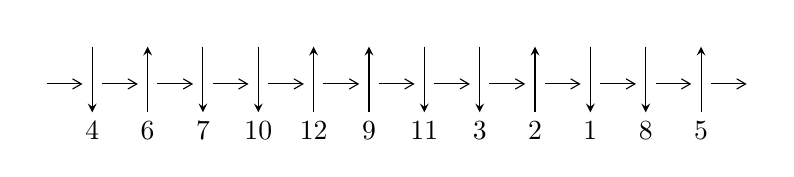
\begin{tikzpicture}[x=20pt, y=17pt]
	% nodes
	\node (C0) at (0, 0) {};
	\node (C1) at (1, 0) {};
	\node (C1U) at (1, +1) {};
	\node (C1D) at (1, -1) {4};

	\node (C2) at (2, 0) {};
	\node (C2U) at (2, +1) {};
	\node (C2D) at (2, -1) {6};

	\node (C3) at (3, 0) {};
	\node (C3U) at (3, +1) {};
	\node (C3D) at (3, -1) {7};

	\node (C4) at (4, 0) {};
	\node (C4U) at (4, +1) {};
	\node (C4D) at (4, -1) {10};

	\node (C5) at (5, 0) {};
	\node (C5U) at (5, +1) {};
	\node (C5D) at (5, -1) {12};

	\node (C6) at (6, 0) {};
	\node (C6U) at (6, +1) {};
	\node (C6D) at (6, -1) {9};

	\node (C7) at (7, 0) {};
	\node (C7U) at (7, +1) {};
	\node (C7D) at (7, -1) {11};

	\node (C8) at (8, 0) {};
	\node (C8U) at (8, +1) {};
	\node (C8D) at (8, -1) {3};

	\node (C9) at (9, 0) {};
	\node (C9U) at (9, +1) {};
	\node (C9D) at (9, -1) {2};

	\node (C10) at (10, 0) {};
	\node (C10U) at (10, +1) {};
	\node (C10D) at (10, -1) {1};

	\node (C11) at (11, 0) {};
	\node (C11U) at (11, +1) {};
	\node (C11D) at (11, -1) {8};

	\node (C12) at (12, 0) {};
	\node (C12U) at (12, +1) {};
	\node (C12D) at (12, -1) {5};
	\node (C13) at (13, 0) {};

	% arrows
	\draw[->,>={angle 60}]
	(C0) edge (C1) (C1) edge (C2) (C2) edge (C3) (C3) edge (C4) (C4) edge (C5) (C5) edge (C6) (C6) edge (C7) (C7) edge (C8) (C8) edge (C9) (C9) edge (C10) (C10) edge (C11) (C11) edge (C12) (C12) edge (C13) ;	\draw[->,>=stealth]
	(C1U) edge (C1D) (C2D) edge (C2U) (C3U) edge (C3D) (C4U) edge (C4D) (C5D) edge (C5U) (C6D) edge (C6U) (C7U) edge (C7D) (C8U) edge (C8D) (C9D) edge (C9U) (C10U) edge (C10D) (C11U) edge (C11D) (C12D) edge (C12U) ;
	\end{tikzpicture} \\
\hhline{~~} \\& 
\textbf{Solving Sequence} \\ \cline{2-2} 
 &
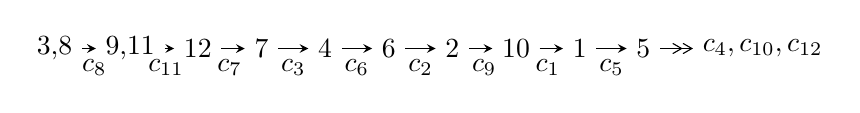
\begin{tikzpicture}[x=23pt, y=7pt]
	% node
	\node (A0) at (-1/8, 0) {3,8};
	\node (A1) at (17/16, 0) {9,11};
	\node (A2) at (17/8, 0) {12};
	\node (A3) at (25/8, 0) {7};
	\node (A4) at (33/8, 0) {4};
	\node (A5) at (41/8, 0) {6};
	\node (A6) at (49/8, 0) {2};
	\node (A7) at (57/8, 0) {10};
	\node (A8) at (65/8, 0) {1};
	\node (A9) at (73/8, 0) {5};
	\node (C1) at (1/2, -1) {$c_{8}$};
	\node (C2) at (13/8, -1) {$c_{11}$};
	\node (C3) at (21/8, -1) {$c_{7}$};
	\node (C4) at (29/8, -1) {$c_{3}$};
	\node (C5) at (37/8, -1) {$c_{6}$};
	\node (C6) at (45/8, -1) {$c_{2}$};
	\node (C7) at (53/8, -1) {$c_{9}$};
	\node (C8) at (61/8, -1) {$c_{1}$};
	\node (C9) at (69/8, -1) {$c_{5}$};
	\node (A10) at (11, 0) {$c_{4},c_{10},c_{12}$};

	% edge
	\draw[->,>=stealth]	
	(A0) edge (A1) (A1) edge (A2) (A2) edge (A3) (A3) edge (A4) (A4) edge (A5) (A5) edge (A6) (A6) edge (A7) (A7) edge (A8) (A8) edge (A9) ;
	\draw[->>,>={angle 60}]	
	(A9) edge (A10);
\end{tikzpicture} \\ 

\end{tabular} \\

\footnotetext{
The image of knot diagram is generated by the software ``\textbf{Draw programme}" developed by Andrew Bartholomew(\url{http://www.layer8.co.uk/maths/draw/index.htm\#Running-draw}), where we modified some parts for our purpose(\url{https://github.com/CATsTAILs/LinksPainter}).
}\phantom \\ \newline 
\centering \textbf{Ideals for irreducible components\footnotemark of $X_{\text{par}}$} 
 
\begin{align*}
I^u_{1}&=\langle 
-8.10959\times10^{2657} u^{208}-3.50955\times10^{2658} u^{207}+\cdots+1.60346\times10^{2656} b+2.47009\times10^{2658},\\
\phantom{I^u_{1}}&\phantom{= \langle  }-4.18869\times10^{2656} u^{208}-1.82159\times10^{2657} u^{207}+\cdots+1.60346\times10^{2656} a+3.34044\times10^{2657},\\
\phantom{I^u_{1}}&\phantom{= \langle  }u^{209}+4 u^{208}+\cdots-29 u+1\rangle \\
I^u_{2}&=\langle 
1.17477\times10^{183} u^{59}-5.87917\times10^{183} u^{58}+\cdots+1.06262\times10^{184} b+6.00821\times10^{183},\\
\phantom{I^u_{2}}&\phantom{= \langle  }-1.29179\times10^{183} u^{59}+6.69835\times10^{183} u^{58}+\cdots+1.06262\times10^{184} a+2.98562\times10^{184},\\
\phantom{I^u_{2}}&\phantom{= \langle  }u^{60}-5 u^{59}+\cdots-2 u+1\rangle \\
\\
\end{align*}
\raggedright * 2 irreducible components of $\dim_{\mathbb{C}}=0$, with total 269 representations.\\
\footnotetext{All coefficients of polynomials are rational numbers. But the coefficients are sometimes approximated in decimal forms when there is not enough margin.}
\newpage
\renewcommand{\arraystretch}{1}
\centering \section*{I. $I^u_{1}= \langle -8.11\times10^{2657} u^{208}-3.51\times10^{2658} u^{207}+\cdots+1.60\times10^{2656} b+2.47\times10^{2658},\;-4.19\times10^{2656} u^{208}-1.82\times10^{2657} u^{207}+\cdots+1.60\times10^{2656} a+3.34\times10^{2657},\;u^{209}+4 u^{208}+\cdots-29 u+1 \rangle$}
\flushleft \textbf{(i) Arc colorings}\\
\begin{tabular}{m{7pt} m{180pt} m{7pt} m{180pt} }
\flushright $a_{3}=$&$\begin{pmatrix}0\\u\end{pmatrix}$ \\
\flushright $a_{8}=$&$\begin{pmatrix}1\\0\end{pmatrix}$ \\
\flushright $a_{9}=$&$\begin{pmatrix}1\\u^2\end{pmatrix}$ \\
\flushright $a_{11}=$&$\begin{pmatrix}2.61228 u^{208}+11.3604 u^{207}+\cdots+180.337 u-20.8327\\50.5754 u^{208}+218.873 u^{207}+\cdots+4014.81 u-154.047\end{pmatrix}$ \\
\flushright $a_{12}=$&$\begin{pmatrix}-47.9632 u^{208}-207.513 u^{207}+\cdots-3834.47 u+133.215\\50.5754 u^{208}+218.873 u^{207}+\cdots+4014.81 u-154.047\end{pmatrix}$ \\
\flushright $a_{7}=$&$\begin{pmatrix}-12.8554 u^{208}-54.2835 u^{207}+\cdots-705.347 u+32.3403\\-35.1135 u^{208}-150.396 u^{207}+\cdots-3067.90 u+121.566\end{pmatrix}$ \\
\flushright $a_{4}=$&$\begin{pmatrix}15.6991 u^{208}+66.6144 u^{207}+\cdots+1787.26 u-69.4800\\36.5093 u^{208}+157.712 u^{207}+\cdots+2975.82 u-113.861\end{pmatrix}$ \\
\flushright $a_{6}=$&$\begin{pmatrix}21.9369 u^{208}+94.9669 u^{207}+\cdots+2292.42 u-86.3643\\-32.2544 u^{208}-138.171 u^{207}+\cdots-2810.34 u+111.485\end{pmatrix}$ \\
\flushright $a_{2}=$&$\begin{pmatrix}-0.0115095 u^{208}-1.71675 u^{207}+\cdots+539.399 u-23.5712\\-21.2435 u^{208}-91.7499 u^{207}+\cdots-1679.37 u+65.8054\end{pmatrix}$ \\
\flushright $a_{10}=$&$\begin{pmatrix}39.6261 u^{208}+171.881 u^{207}+\cdots+3100.82 u-107.250\\-19.3332 u^{208}-83.3766 u^{207}+\cdots-1615.68 u+62.4346\end{pmatrix}$ \\
\flushright $a_{1}=$&$\begin{pmatrix}29.0576 u^{208}+124.992 u^{207}+\cdots+2371.98 u-105.034\\25.8012 u^{208}+111.596 u^{207}+\cdots+2077.10 u-79.6954\end{pmatrix}$ \\
\flushright $a_{5}=$&$\begin{pmatrix}-5.04414 u^{208}-22.4581 u^{207}+\cdots-299.878 u+11.0691\\4.32188 u^{208}+18.7946 u^{207}+\cdots+329.949 u-12.6917\end{pmatrix}$\\&\end{tabular}
\flushleft \textbf{(ii) Obstruction class $= -1$}\\~\\
\flushleft \textbf{(iii) Cusp Shapes $= -339.908 u^{208}-1483.97 u^{207}+\cdots-23747.8 u+897.796$}\\~\\
\newpage\renewcommand{\arraystretch}{1}
\flushleft \textbf{(iv) u-Polynomials at the component}\newline \\
\begin{tabular}{m{50pt}|m{274pt}}
Crossings & \hspace{64pt}u-Polynomials at each crossing \\
\hline $$\begin{aligned}c_{1}\end{aligned}$$&$\begin{aligned}
&u^{209}+16 u^{208}+\cdots-229 u+7
\end{aligned}$\\
\hline $$\begin{aligned}c_{2}\end{aligned}$$&$\begin{aligned}
&u^{209}+20 u^{207}+\cdots+1001187 u+56817
\end{aligned}$\\
\hline $$\begin{aligned}c_{3}\end{aligned}$$&$\begin{aligned}
&u^{209}+8 u^{208}+\cdots+10140313539 u-1878370717
\end{aligned}$\\
\hline $$\begin{aligned}c_{4}\end{aligned}$$&$\begin{aligned}
&u^{209}-5 u^{208}+\cdots+4624338 u-184123
\end{aligned}$\\
\hline $$\begin{aligned}c_{5},c_{12}\end{aligned}$$&$\begin{aligned}
&u^{209}+u^{208}+\cdots+4331046357 u+113222443
\end{aligned}$\\
\hline $$\begin{aligned}c_{6}\end{aligned}$$&$\begin{aligned}
&u^{209}+16 u^{208}+\cdots+12 u+1
\end{aligned}$\\
\hline $$\begin{aligned}c_{7},c_{11}\end{aligned}$$&$\begin{aligned}
&u^{209}+4 u^{208}+\cdots+2657560 u+2311849
\end{aligned}$\\
\hline $$\begin{aligned}c_{8}\end{aligned}$$&$\begin{aligned}
&u^{209}+4 u^{208}+\cdots-29 u+1
\end{aligned}$\\
\hline $$\begin{aligned}c_{9}\end{aligned}$$&$\begin{aligned}
&u^{209}+45 u^{207}+\cdots+739402858830 u+26116631329
\end{aligned}$\\
\hline $$\begin{aligned}c_{10}\end{aligned}$$&$\begin{aligned}
&u^{209}-7 u^{208}+\cdots-17609 u+341
\end{aligned}$\\
\hline
\end{tabular}\\~\\
\newpage\renewcommand{\arraystretch}{1}
\flushleft \textbf{(v) Riley Polynomials at the component}\newline \\
\begin{tabular}{m{50pt}|m{274pt}}
Crossings & \hspace{64pt}Riley Polynomials at each crossing \\
\hline $$\begin{aligned}c_{1}\end{aligned}$$&$\begin{aligned}
&y^{209}-2 y^{208}+\cdots-6625 y-49
\end{aligned}$\\
\hline $$\begin{aligned}c_{2}\end{aligned}$$&$\begin{aligned}
&y^{209}+40 y^{208}+\cdots-266988642255 y-3228171489
\end{aligned}$\\
\hline $$\begin{aligned}c_{3}\end{aligned}$$&$\begin{aligned}
&y^{209}-8 y^{208}+\cdots+2.14\times10^{20} y-3.53\times10^{18}
\end{aligned}$\\
\hline $$\begin{aligned}c_{4}\end{aligned}$$&$\begin{aligned}
&y^{209}-47 y^{208}+\cdots+8724659978546 y-33901279129
\end{aligned}$\\
\hline $$\begin{aligned}c_{5},c_{12}\end{aligned}$$&$\begin{aligned}
&y^{209}+165 y^{208}+\cdots+833990559064792201 y-12819321598888249
\end{aligned}$\\
\hline $$\begin{aligned}c_{6}\end{aligned}$$&$\begin{aligned}
&y^{209}+30 y^{208}+\cdots-56 y-1
\end{aligned}$\\
\hline $$\begin{aligned}c_{7},c_{11}\end{aligned}$$&$\begin{aligned}
&y^{209}-118 y^{208}+\cdots+340566951866202 y-5344645798801
\end{aligned}$\\
\hline $$\begin{aligned}c_{8}\end{aligned}$$&$\begin{aligned}
&y^{209}-8 y^{208}+\cdots-1269 y-1
\end{aligned}$\\
\hline $$\begin{aligned}c_{9}\end{aligned}$$&$\begin{aligned}
&y^{209}+90 y^{208}+\cdots-4.99\times10^{22} y-6.82\times10^{20}
\end{aligned}$\\
\hline $$\begin{aligned}c_{10}\end{aligned}$$&$\begin{aligned}
&y^{209}-37 y^{208}+\cdots+35347503 y-116281
\end{aligned}$\\
\hline
\end{tabular}\\~\\
\newpage\flushleft \textbf{(vi) Complex Volumes and Cusp Shapes}
$$\begin{array}{c|c|c}  
\text{Solutions to }I^u_{1}& \I (\text{vol} + \sqrt{-1}CS) & \text{Cusp shape}\\
 \hline 
\begin{aligned}
u &= -0.322396 + 0.941816 I \\
a &= \phantom{-}1.078060 - 0.213369 I \\
b &= -0.766823 + 0.134796 I\end{aligned}
 & -4.12956 + 5.33084 I & \phantom{-0.000000 } 0 \\ \hline\begin{aligned}
u &= -0.322396 - 0.941816 I \\
a &= \phantom{-}1.078060 + 0.213369 I \\
b &= -0.766823 - 0.134796 I\end{aligned}
 & -4.12956 - 5.33084 I & \phantom{-0.000000 } 0 \\ \hline\begin{aligned}
u &= \phantom{-}0.688925 + 0.735337 I \\
a &= -2.12587 + 0.58108 I \\
b &= -1.251480 - 0.234975 I\end{aligned}
 & -6.95554 - 5.82618 I & \phantom{-0.000000 } 0 \\ \hline\begin{aligned}
u &= \phantom{-}0.688925 - 0.735337 I \\
a &= -2.12587 - 0.58108 I \\
b &= -1.251480 + 0.234975 I\end{aligned}
 & -6.95554 + 5.82618 I & \phantom{-0.000000 } 0 \\ \hline\begin{aligned}
u &= -0.466678 + 0.900813 I \\
a &= \phantom{-}0.457825 + 0.401507 I \\
b &= \phantom{-}0.605901 - 0.696082 I\end{aligned}
 & \phantom{-}0.41107 + 1.81059 I & \phantom{-0.000000 } 0 \\ \hline\begin{aligned}
u &= -0.466678 - 0.900813 I \\
a &= \phantom{-}0.457825 - 0.401507 I \\
b &= \phantom{-}0.605901 + 0.696082 I\end{aligned}
 & \phantom{-}0.41107 - 1.81059 I & \phantom{-0.000000 } 0 \\ \hline\begin{aligned}
u &= -0.295002 + 0.983333 I \\
a &= -0.979898 + 0.538820 I \\
b &= \phantom{-}1.062930 + 0.226140 I\end{aligned}
 & \phantom{-}0.24315 + 2.45125 I & \phantom{-0.000000 } 0 \\ \hline\begin{aligned}
u &= -0.295002 - 0.983333 I \\
a &= -0.979898 - 0.538820 I \\
b &= \phantom{-}1.062930 - 0.226140 I\end{aligned}
 & \phantom{-}0.24315 - 2.45125 I & \phantom{-0.000000 } 0 \\ \hline\begin{aligned}
u &= \phantom{-}0.491065 + 0.809479 I \\
a &= \phantom{-}0.52229 - 1.70212 I \\
b &= \phantom{-}1.166850 + 0.481470 I\end{aligned}
 & -3.68167 - 7.05122 I & \phantom{-0.000000 } 0 \\ \hline\begin{aligned}
u &= \phantom{-}0.491065 - 0.809479 I \\
a &= \phantom{-}0.52229 + 1.70212 I \\
b &= \phantom{-}1.166850 - 0.481470 I\end{aligned}
 & -3.68167 + 7.05122 I & \phantom{-0.000000 } 0\\
 \hline 
 \end{array}$$\newpage$$\begin{array}{c|c|c}  
\text{Solutions to }I^u_{1}& \I (\text{vol} + \sqrt{-1}CS) & \text{Cusp shape}\\
 \hline 
\begin{aligned}
u &= \phantom{-}1.035890 + 0.197559 I \\
a &= -0.977539 + 0.294685 I \\
b &= -1.45275 - 0.37250 I\end{aligned}
 & -7.67423 + 1.32305 I & \phantom{-0.000000 } 0 \\ \hline\begin{aligned}
u &= \phantom{-}1.035890 - 0.197559 I \\
a &= -0.977539 - 0.294685 I \\
b &= -1.45275 + 0.37250 I\end{aligned}
 & -7.67423 - 1.32305 I & \phantom{-0.000000 } 0 \\ \hline\begin{aligned}
u &= \phantom{-}0.909494 + 0.536845 I \\
a &= \phantom{-}0.592526 - 0.548109 I \\
b &= \phantom{-}0.057360 + 0.567159 I\end{aligned}
 & -0.36766 + 3.81034 I & \phantom{-0.000000 } 0 \\ \hline\begin{aligned}
u &= \phantom{-}0.909494 - 0.536845 I \\
a &= \phantom{-}0.592526 + 0.548109 I \\
b &= \phantom{-}0.057360 - 0.567159 I\end{aligned}
 & -0.36766 - 3.81034 I & \phantom{-0.000000 } 0 \\ \hline\begin{aligned}
u &= \phantom{-}0.629677 + 0.700527 I \\
a &= -1.88696 + 1.75127 I \\
b &= -0.917287 - 0.597759 I\end{aligned}
 & -1.68445 - 7.10492 I & \phantom{-0.000000 } 0 \\ \hline\begin{aligned}
u &= \phantom{-}0.629677 - 0.700527 I \\
a &= -1.88696 - 1.75127 I \\
b &= -0.917287 + 0.597759 I\end{aligned}
 & -1.68445 + 7.10492 I & \phantom{-0.000000 } 0 \\ \hline\begin{aligned}
u &= \phantom{-}0.669692 + 0.832374 I \\
a &= -0.080351 - 1.150370 I \\
b &= \phantom{-}0.737976 + 0.128827 I\end{aligned}
 & -6.00830 - 5.33123 I & \phantom{-0.000000 } 0 \\ \hline\begin{aligned}
u &= \phantom{-}0.669692 - 0.832374 I \\
a &= -0.080351 + 1.150370 I \\
b &= \phantom{-}0.737976 - 0.128827 I\end{aligned}
 & -6.00830 + 5.33123 I & \phantom{-0.000000 } 0 \\ \hline\begin{aligned}
u &= -1.057120 + 0.161356 I \\
a &= -0.326208 + 0.027726 I \\
b &= -0.57041 - 1.41267 I\end{aligned}
 & -1.82198 - 3.52569 I & \phantom{-0.000000 } 0 \\ \hline\begin{aligned}
u &= -1.057120 - 0.161356 I \\
a &= -0.326208 - 0.027726 I \\
b &= -0.57041 + 1.41267 I\end{aligned}
 & -1.82198 + 3.52569 I & \phantom{-0.000000 } 0\\
 \hline 
 \end{array}$$\newpage$$\begin{array}{c|c|c}  
\text{Solutions to }I^u_{1}& \I (\text{vol} + \sqrt{-1}CS) & \text{Cusp shape}\\
 \hline 
\begin{aligned}
u &= \phantom{-}0.684254 + 0.842297 I \\
a &= \phantom{-}1.70966 - 0.98842 I \\
b &= \phantom{-}1.001110 + 0.102873 I\end{aligned}
 & -5.12674 - 2.17128 I & \phantom{-0.000000 } 0 \\ \hline\begin{aligned}
u &= \phantom{-}0.684254 - 0.842297 I \\
a &= \phantom{-}1.70966 + 0.98842 I \\
b &= \phantom{-}1.001110 - 0.102873 I\end{aligned}
 & -5.12674 + 2.17128 I & \phantom{-0.000000 } 0 \\ \hline\begin{aligned}
u &= -0.778986 + 0.473422 I \\
a &= -0.830172 - 0.538918 I \\
b &= \phantom{-}0.034639 + 0.766751 I\end{aligned}
 & -0.52177 + 2.57685 I & \phantom{-0.000000 } 0 \\ \hline\begin{aligned}
u &= -0.778986 - 0.473422 I \\
a &= -0.830172 + 0.538918 I \\
b &= \phantom{-}0.034639 - 0.766751 I\end{aligned}
 & -0.52177 - 2.57685 I & \phantom{-0.000000 } 0 \\ \hline\begin{aligned}
u &= \phantom{-}0.664235 + 0.602411 I \\
a &= -0.085565 + 0.192954 I \\
b &= -0.272651 - 1.117750 I\end{aligned}
 & \phantom{-}1.23843 - 4.89844 I & \phantom{-0.000000 } 0 \\ \hline\begin{aligned}
u &= \phantom{-}0.664235 - 0.602411 I \\
a &= -0.085565 - 0.192954 I \\
b &= -0.272651 + 1.117750 I\end{aligned}
 & \phantom{-}1.23843 + 4.89844 I & \phantom{-0.000000 } 0 \\ \hline\begin{aligned}
u &= -0.170528 + 0.868979 I \\
a &= -0.346178 - 0.206792 I \\
b &= \phantom{-}0.060765 + 0.793071 I\end{aligned}
 & -1.02684 + 1.21925 I & \phantom{-0.000000 } 0 \\ \hline\begin{aligned}
u &= -0.170528 - 0.868979 I \\
a &= -0.346178 + 0.206792 I \\
b &= \phantom{-}0.060765 - 0.793071 I\end{aligned}
 & -1.02684 - 1.21925 I & \phantom{-0.000000 } 0 \\ \hline\begin{aligned}
u &= \phantom{-}0.702475 + 0.535536 I \\
a &= \phantom{-}2.13084 - 1.02466 I \\
b &= \phantom{-}1.214860 + 0.463350 I\end{aligned}
 & -4.04158 - 5.84535 I & \phantom{-0.000000 } 0 \\ \hline\begin{aligned}
u &= \phantom{-}0.702475 - 0.535536 I \\
a &= \phantom{-}2.13084 + 1.02466 I \\
b &= \phantom{-}1.214860 - 0.463350 I\end{aligned}
 & -4.04158 + 5.84535 I & \phantom{-0.000000 } 0\\
 \hline 
 \end{array}$$\newpage$$\begin{array}{c|c|c}  
\text{Solutions to }I^u_{1}& \I (\text{vol} + \sqrt{-1}CS) & \text{Cusp shape}\\
 \hline 
\begin{aligned}
u &= -0.645436 + 0.601214 I \\
a &= \phantom{-}1.32439 + 0.58808 I \\
b &= \phantom{-}1.39035 - 0.75314 I\end{aligned}
 & -6.3552 + 13.4802 I & \phantom{-0.000000 } 0 \\ \hline\begin{aligned}
u &= -0.645436 - 0.601214 I \\
a &= \phantom{-}1.32439 - 0.58808 I \\
b &= \phantom{-}1.39035 + 0.75314 I\end{aligned}
 & -6.3552 - 13.4802 I & \phantom{-0.000000 } 0 \\ \hline\begin{aligned}
u &= \phantom{-}0.808900 + 0.349105 I \\
a &= -1.40992 + 0.29775 I \\
b &= -1.47742 - 0.81750 I\end{aligned}
 & -4.62811 - 4.87068 I & \phantom{-0.000000 } 0 \\ \hline\begin{aligned}
u &= \phantom{-}0.808900 - 0.349105 I \\
a &= -1.40992 - 0.29775 I \\
b &= -1.47742 + 0.81750 I\end{aligned}
 & -4.62811 + 4.87068 I & \phantom{-0.000000 } 0 \\ \hline\begin{aligned}
u &= -0.629684 + 0.614199 I \\
a &= \phantom{-}0.391089 - 0.612087 I \\
b &= -0.556757 - 0.560991 I\end{aligned}
 & -0.72140 + 2.54607 I & \phantom{-0.000000 } 0 \\ \hline\begin{aligned}
u &= -0.629684 - 0.614199 I \\
a &= \phantom{-}0.391089 + 0.612087 I \\
b &= -0.556757 + 0.560991 I\end{aligned}
 & -0.72140 - 2.54607 I & \phantom{-0.000000 } 0 \\ \hline\begin{aligned}
u &= -1.13018\phantom{ +0.000000I} \\
a &= -1.24879\phantom{ +0.000000I} \\
b &= -1.26027\phantom{ +0.000000I}\end{aligned}
 & -2.54194\phantom{ +0.000000I} & \phantom{-0.000000 } 0 \\ \hline\begin{aligned}
u &= \phantom{-}0.509588 + 0.696373 I \\
a &= \phantom{-}1.65326 - 0.94616 I \\
b &= \phantom{-}1.283870 + 0.477392 I\end{aligned}
 & -4.83547 - 5.83889 I & \phantom{-0.000000 } 0 \\ \hline\begin{aligned}
u &= \phantom{-}0.509588 - 0.696373 I \\
a &= \phantom{-}1.65326 + 0.94616 I \\
b &= \phantom{-}1.283870 - 0.477392 I\end{aligned}
 & -4.83547 + 5.83889 I & \phantom{-0.000000 } 0 \\ \hline\begin{aligned}
u &= -0.324124 + 1.094780 I \\
a &= -0.405834 + 0.280821 I \\
b &= \phantom{-}0.864367 + 0.041365 I\end{aligned}
 & \phantom{-}0.38083 + 2.95440 I & \phantom{-0.000000 } 0\\
 \hline 
 \end{array}$$\newpage$$\begin{array}{c|c|c}  
\text{Solutions to }I^u_{1}& \I (\text{vol} + \sqrt{-1}CS) & \text{Cusp shape}\\
 \hline 
\begin{aligned}
u &= -0.324124 - 1.094780 I \\
a &= -0.405834 - 0.280821 I \\
b &= \phantom{-}0.864367 - 0.041365 I\end{aligned}
 & \phantom{-}0.38083 - 2.95440 I & \phantom{-0.000000 } 0 \\ \hline\begin{aligned}
u &= -1.127800 + 0.184799 I \\
a &= \phantom{-}1.51057 + 0.77910 I \\
b &= \phantom{-}1.118360 + 0.319243 I\end{aligned}
 & -8.37201 - 0.61813 I & \phantom{-0.000000 } 0 \\ \hline\begin{aligned}
u &= -1.127800 - 0.184799 I \\
a &= \phantom{-}1.51057 - 0.77910 I \\
b &= \phantom{-}1.118360 - 0.319243 I\end{aligned}
 & -8.37201 + 0.61813 I & \phantom{-0.000000 } 0 \\ \hline\begin{aligned}
u &= -0.523025 + 1.017600 I \\
a &= -0.237001 + 0.429116 I \\
b &= \phantom{-}0.669239 + 0.319052 I\end{aligned}
 & \phantom{-}0.27896 + 2.84359 I & \phantom{-0.000000 } 0 \\ \hline\begin{aligned}
u &= -0.523025 - 1.017600 I \\
a &= -0.237001 - 0.429116 I \\
b &= \phantom{-}0.669239 - 0.319052 I\end{aligned}
 & \phantom{-}0.27896 - 2.84359 I & \phantom{-0.000000 } 0 \\ \hline\begin{aligned}
u &= \phantom{-}0.170881 + 0.834356 I \\
a &= -0.366988 + 0.118463 I \\
b &= \phantom{-}0.202472 + 0.688941 I\end{aligned}
 & \phantom{-}3.46797 + 1.79940 I & \phantom{-0.000000 } 0 \\ \hline\begin{aligned}
u &= \phantom{-}0.170881 - 0.834356 I \\
a &= -0.366988 - 0.118463 I \\
b &= \phantom{-}0.202472 - 0.688941 I\end{aligned}
 & \phantom{-}3.46797 - 1.79940 I & \phantom{-0.000000 } 0 \\ \hline\begin{aligned}
u &= \phantom{-}0.058309 + 0.838997 I \\
a &= \phantom{-}0.584408 - 0.004947 I \\
b &= \phantom{-}0.835937 - 0.827738 I\end{aligned}
 & -0.17588 + 3.87813 I & \phantom{-0.000000 } 0 \\ \hline\begin{aligned}
u &= \phantom{-}0.058309 - 0.838997 I \\
a &= \phantom{-}0.584408 + 0.004947 I \\
b &= \phantom{-}0.835937 + 0.827738 I\end{aligned}
 & -0.17588 - 3.87813 I & \phantom{-0.000000 } 0 \\ \hline\begin{aligned}
u &= -1.065600 + 0.484501 I \\
a &= \phantom{-}1.79052 - 0.01229 I \\
b &= \phantom{-}1.237350 - 0.267508 I\end{aligned}
 & -8.93721 + 6.04392 I & \phantom{-0.000000 } 0\\
 \hline 
 \end{array}$$\newpage$$\begin{array}{c|c|c}  
\text{Solutions to }I^u_{1}& \I (\text{vol} + \sqrt{-1}CS) & \text{Cusp shape}\\
 \hline 
\begin{aligned}
u &= -1.065600 - 0.484501 I \\
a &= \phantom{-}1.79052 + 0.01229 I \\
b &= \phantom{-}1.237350 + 0.267508 I\end{aligned}
 & -8.93721 - 6.04392 I & \phantom{-0.000000 } 0 \\ \hline\begin{aligned}
u &= \phantom{-}1.171450 + 0.184950 I \\
a &= -1.56947 + 0.52835 I \\
b &= -1.108940 + 0.402672 I\end{aligned}
 & -7.47840 + 2.37028 I & \phantom{-0.000000 } 0 \\ \hline\begin{aligned}
u &= \phantom{-}1.171450 - 0.184950 I \\
a &= -1.56947 - 0.52835 I \\
b &= -1.108940 - 0.402672 I\end{aligned}
 & -7.47840 - 2.37028 I & \phantom{-0.000000 } 0 \\ \hline\begin{aligned}
u &= -0.541897 + 0.600862 I \\
a &= -1.097950 - 0.794729 I \\
b &= -1.33090 + 0.60363 I\end{aligned}
 & -6.04307 + 4.07584 I & \phantom{-0.000000 } 0 \\ \hline\begin{aligned}
u &= -0.541897 - 0.600862 I \\
a &= -1.097950 + 0.794729 I \\
b &= -1.33090 - 0.60363 I\end{aligned}
 & -6.04307 - 4.07584 I & \phantom{-0.000000 } 0 \\ \hline\begin{aligned}
u &= -0.206432 + 1.175830 I \\
a &= -0.045813 + 0.308018 I \\
b &= -0.734888 + 0.220198 I\end{aligned}
 & -1.02960 + 3.25121 I & \phantom{-0.000000 } 0 \\ \hline\begin{aligned}
u &= -0.206432 - 1.175830 I \\
a &= -0.045813 - 0.308018 I \\
b &= -0.734888 - 0.220198 I\end{aligned}
 & -1.02960 - 3.25121 I & \phantom{-0.000000 } 0 \\ \hline\begin{aligned}
u &= -0.528057 + 0.591427 I \\
a &= -0.691390 - 0.251399 I \\
b &= -0.464598 + 0.503732 I\end{aligned}
 & -0.94301 + 1.39215 I & \phantom{-0.000000 } 0 \\ \hline\begin{aligned}
u &= -0.528057 - 0.591427 I \\
a &= -0.691390 + 0.251399 I \\
b &= -0.464598 - 0.503732 I\end{aligned}
 & -0.94301 - 1.39215 I & \phantom{-0.000000 } 0 \\ \hline\begin{aligned}
u &= -0.781626 + 0.129198 I \\
a &= -3.14009 + 0.40454 I \\
b &= -1.190240 + 0.476110 I\end{aligned}
 & -7.16288 + 11.23080 I & \phantom{-0.000000 } 0\\
 \hline 
 \end{array}$$\newpage$$\begin{array}{c|c|c}  
\text{Solutions to }I^u_{1}& \I (\text{vol} + \sqrt{-1}CS) & \text{Cusp shape}\\
 \hline 
\begin{aligned}
u &= -0.781626 - 0.129198 I \\
a &= -3.14009 - 0.40454 I \\
b &= -1.190240 - 0.476110 I\end{aligned}
 & -7.16288 - 11.23080 I & \phantom{-0.000000 } 0 \\ \hline\begin{aligned}
u &= \phantom{-}0.106093 + 0.780214 I \\
a &= \phantom{-}1.90788 + 0.87396 I \\
b &= -1.203160 - 0.350716 I\end{aligned}
 & -5.28742 - 11.13400 I & \phantom{-0.000000 } 0 \\ \hline\begin{aligned}
u &= \phantom{-}0.106093 - 0.780214 I \\
a &= \phantom{-}1.90788 - 0.87396 I \\
b &= -1.203160 + 0.350716 I\end{aligned}
 & -5.28742 + 11.13400 I & \phantom{-0.000000 } 0 \\ \hline\begin{aligned}
u &= -0.755053 + 0.171762 I \\
a &= -0.980882 - 0.379650 I \\
b &= \phantom{-}0.029016 - 0.473614 I\end{aligned}
 & -4.57808 - 1.05851 I & \phantom{-0.000000 } 0 \\ \hline\begin{aligned}
u &= -0.755053 - 0.171762 I \\
a &= -0.980882 + 0.379650 I \\
b &= \phantom{-}0.029016 + 0.473614 I\end{aligned}
 & -4.57808 + 1.05851 I & \phantom{-0.000000 } 0 \\ \hline\begin{aligned}
u &= -0.763634 + 0.116736 I \\
a &= -1.198410 - 0.196738 I \\
b &= -1.237830 + 0.539694 I\end{aligned}
 & -2.42927 + 1.02706 I & \phantom{-0.000000 } 0 \\ \hline\begin{aligned}
u &= -0.763634 - 0.116736 I \\
a &= -1.198410 + 0.196738 I \\
b &= -1.237830 - 0.539694 I\end{aligned}
 & -2.42927 - 1.02706 I & \phantom{-0.000000 } 0 \\ \hline\begin{aligned}
u &= -0.054084 + 0.764953 I \\
a &= -0.660638 + 1.153620 I \\
b &= \phantom{-}0.792541 - 0.465137 I\end{aligned}
 & \phantom{-}1.59684 + 2.06914 I & \phantom{-0.000000 } 0 \\ \hline\begin{aligned}
u &= -0.054084 - 0.764953 I \\
a &= -0.660638 - 1.153620 I \\
b &= \phantom{-}0.792541 + 0.465137 I\end{aligned}
 & \phantom{-}1.59684 - 2.06914 I & \phantom{-0.000000 } 0 \\ \hline\begin{aligned}
u &= -0.866749 + 0.877622 I \\
a &= \phantom{-}0.150703 - 0.082080 I \\
b &= \phantom{-}0.101478 + 0.884405 I\end{aligned}
 & -3.29272 + 6.59289 I & \phantom{-0.000000 } 0\\
 \hline 
 \end{array}$$\newpage$$\begin{array}{c|c|c}  
\text{Solutions to }I^u_{1}& \I (\text{vol} + \sqrt{-1}CS) & \text{Cusp shape}\\
 \hline 
\begin{aligned}
u &= -0.866749 - 0.877622 I \\
a &= \phantom{-}0.150703 + 0.082080 I \\
b &= \phantom{-}0.101478 - 0.884405 I\end{aligned}
 & -3.29272 - 6.59289 I & \phantom{-0.000000 } 0 \\ \hline\begin{aligned}
u &= -0.726304 + 1.000820 I \\
a &= -0.328436 + 0.144576 I \\
b &= \phantom{-}0.457951 + 1.017620 I\end{aligned}
 & \phantom{-}0.49729 + 3.11019 I & \phantom{-0.000000 } 0 \\ \hline\begin{aligned}
u &= -0.726304 - 1.000820 I \\
a &= -0.328436 - 0.144576 I \\
b &= \phantom{-}0.457951 - 1.017620 I\end{aligned}
 & \phantom{-}0.49729 - 3.11019 I & \phantom{-0.000000 } 0 \\ \hline\begin{aligned}
u &= -0.000760 + 0.760636 I \\
a &= \phantom{-}2.40210 + 0.01528 I \\
b &= -0.886866 + 0.198642 I\end{aligned}
 & \phantom{-}0.67024 + 4.87492 I & \phantom{-0.000000 } 0 \\ \hline\begin{aligned}
u &= -0.000760 - 0.760636 I \\
a &= \phantom{-}2.40210 - 0.01528 I \\
b &= -0.886866 - 0.198642 I\end{aligned}
 & \phantom{-}0.67024 - 4.87492 I & \phantom{-0.000000 } 0 \\ \hline\begin{aligned}
u &= \phantom{-}0.779227 + 0.982253 I \\
a &= \phantom{-}0.062814 + 0.165899 I \\
b &= \phantom{-}0.380044 - 0.921225 I\end{aligned}
 & \phantom{-}3.78269 - 2.72916 I & \phantom{-0.000000 } 0 \\ \hline\begin{aligned}
u &= \phantom{-}0.779227 - 0.982253 I \\
a &= \phantom{-}0.062814 - 0.165899 I \\
b &= \phantom{-}0.380044 + 0.921225 I\end{aligned}
 & \phantom{-}3.78269 + 2.72916 I & \phantom{-0.000000 } 0 \\ \hline\begin{aligned}
u &= -0.965297 + 0.807005 I \\
a &= \phantom{-}1.78691 + 0.92455 I \\
b &= \phantom{-}0.724314 - 0.740370 I\end{aligned}
 & -0.80196 + 8.84500 I & \phantom{-0.000000 } 0 \\ \hline\begin{aligned}
u &= -0.965297 - 0.807005 I \\
a &= \phantom{-}1.78691 - 0.92455 I \\
b &= \phantom{-}0.724314 + 0.740370 I\end{aligned}
 & -0.80196 - 8.84500 I & \phantom{-0.000000 } 0 \\ \hline\begin{aligned}
u &= \phantom{-}0.586580 + 0.439517 I \\
a &= \phantom{-}0.87193 - 2.03254 I \\
b &= \phantom{-}1.017320 + 0.497045 I\end{aligned}
 & -6.81632 - 4.67724 I & \phantom{-0.000000 } 0\\
 \hline 
 \end{array}$$\newpage$$\begin{array}{c|c|c}  
\text{Solutions to }I^u_{1}& \I (\text{vol} + \sqrt{-1}CS) & \text{Cusp shape}\\
 \hline 
\begin{aligned}
u &= \phantom{-}0.586580 - 0.439517 I \\
a &= \phantom{-}0.87193 + 2.03254 I \\
b &= \phantom{-}1.017320 - 0.497045 I\end{aligned}
 & -6.81632 + 4.67724 I & \phantom{-0.000000 } 0 \\ \hline\begin{aligned}
u &= -0.491431 + 0.540049 I \\
a &= -0.486115 - 1.192940 I \\
b &= -1.106500 + 0.760056 I\end{aligned}
 & -5.60199 + 6.65769 I & \phantom{-0.000000 } 0 \\ \hline\begin{aligned}
u &= -0.491431 - 0.540049 I \\
a &= -0.486115 + 1.192940 I \\
b &= -1.106500 - 0.760056 I\end{aligned}
 & -5.60199 - 6.65769 I & \phantom{-0.000000 } 0 \\ \hline\begin{aligned}
u &= \phantom{-}0.749807 + 1.040040 I \\
a &= \phantom{-}0.179131 - 0.036316 I \\
b &= -0.221447 + 0.877552 I\end{aligned}
 & \phantom{-}1.12746 - 9.87504 I & \phantom{-0.000000 } 0 \\ \hline\begin{aligned}
u &= \phantom{-}0.749807 - 1.040040 I \\
a &= \phantom{-}0.179131 + 0.036316 I \\
b &= -0.221447 - 0.877552 I\end{aligned}
 & \phantom{-}1.12746 + 9.87504 I & \phantom{-0.000000 } 0 \\ \hline\begin{aligned}
u &= -1.211380 + 0.428496 I \\
a &= \phantom{-}1.086930 - 0.170859 I \\
b &= \phantom{-}1.284470 + 0.371708 I\end{aligned}
 & -9.29642 + 2.85337 I & \phantom{-0.000000 } 0 \\ \hline\begin{aligned}
u &= -1.211380 - 0.428496 I \\
a &= \phantom{-}1.086930 + 0.170859 I \\
b &= \phantom{-}1.284470 - 0.371708 I\end{aligned}
 & -9.29642 - 2.85337 I & \phantom{-0.000000 } 0 \\ \hline\begin{aligned}
u &= -1.144490 + 0.596072 I \\
a &= -1.394560 - 0.220003 I \\
b &= -1.58038 + 0.07420 I\end{aligned}
 & -11.74990 - 0.76353 I & \phantom{-0.000000 } 0 \\ \hline\begin{aligned}
u &= -1.144490 - 0.596072 I \\
a &= -1.394560 + 0.220003 I \\
b &= -1.58038 - 0.07420 I\end{aligned}
 & -11.74990 + 0.76353 I & \phantom{-0.000000 } 0 \\ \hline\begin{aligned}
u &= -0.356131 + 0.599507 I \\
a &= -0.781460 + 0.167908 I \\
b &= -0.033703 + 0.651955 I\end{aligned}
 & -0.49466 + 1.57044 I & \phantom{-0.000000 } 0\\
 \hline 
 \end{array}$$\newpage$$\begin{array}{c|c|c}  
\text{Solutions to }I^u_{1}& \I (\text{vol} + \sqrt{-1}CS) & \text{Cusp shape}\\
 \hline 
\begin{aligned}
u &= -0.356131 - 0.599507 I \\
a &= -0.781460 - 0.167908 I \\
b &= -0.033703 - 0.651955 I\end{aligned}
 & -0.49466 - 1.57044 I & \phantom{-0.000000 } 0 \\ \hline\begin{aligned}
u &= \phantom{-}1.300980 + 0.077838 I \\
a &= \phantom{-}1.71807 - 0.61544 I \\
b &= \phantom{-}0.703123 - 0.066080 I\end{aligned}
 & -6.24661 + 1.36052 I & \phantom{-0.000000 } 0 \\ \hline\begin{aligned}
u &= \phantom{-}1.300980 - 0.077838 I \\
a &= \phantom{-}1.71807 + 0.61544 I \\
b &= \phantom{-}0.703123 + 0.066080 I\end{aligned}
 & -6.24661 - 1.36052 I & \phantom{-0.000000 } 0 \\ \hline\begin{aligned}
u &= -0.242624 + 0.642130 I \\
a &= \phantom{-}1.233290 + 0.278528 I \\
b &= -0.314217 + 0.677082 I\end{aligned}
 & \phantom{-}2.04033 + 4.97528 I & \phantom{-0.000000 } 0 \\ \hline\begin{aligned}
u &= -0.242624 - 0.642130 I \\
a &= \phantom{-}1.233290 - 0.278528 I \\
b &= -0.314217 - 0.677082 I\end{aligned}
 & \phantom{-}2.04033 - 4.97528 I & \phantom{-0.000000 } 0 \\ \hline\begin{aligned}
u &= \phantom{-}1.114240 + 0.721512 I \\
a &= -0.777343 + 0.487861 I \\
b &= -0.708900 - 1.039380 I\end{aligned}
 & -2.69324 - 4.70021 I & \phantom{-0.000000 } 0 \\ \hline\begin{aligned}
u &= \phantom{-}1.114240 - 0.721512 I \\
a &= -0.777343 - 0.487861 I \\
b &= -0.708900 + 1.039380 I\end{aligned}
 & -2.69324 + 4.70021 I & \phantom{-0.000000 } 0 \\ \hline\begin{aligned}
u &= \phantom{-}1.164070 + 0.641233 I \\
a &= \phantom{-}1.78988 - 0.01138 I \\
b &= \phantom{-}0.833987 + 0.192797 I\end{aligned}
 & \phantom{-}0.23188 - 5.10410 I & \phantom{-0.000000 } 0 \\ \hline\begin{aligned}
u &= \phantom{-}1.164070 - 0.641233 I \\
a &= \phantom{-}1.78988 + 0.01138 I \\
b &= \phantom{-}0.833987 - 0.192797 I\end{aligned}
 & \phantom{-}0.23188 + 5.10410 I & \phantom{-0.000000 } 0 \\ \hline\begin{aligned}
u &= -1.192820 + 0.629157 I \\
a &= \phantom{-}0.149440 - 0.304496 I \\
b &= \phantom{-}0.213744 + 1.238980 I\end{aligned}
 & \phantom{-}0.80140 + 5.95799 I & \phantom{-0.000000 } 0\\
 \hline 
 \end{array}$$\newpage$$\begin{array}{c|c|c}  
\text{Solutions to }I^u_{1}& \I (\text{vol} + \sqrt{-1}CS) & \text{Cusp shape}\\
 \hline 
\begin{aligned}
u &= -1.192820 - 0.629157 I \\
a &= \phantom{-}0.149440 + 0.304496 I \\
b &= \phantom{-}0.213744 - 1.238980 I\end{aligned}
 & \phantom{-}0.80140 - 5.95799 I & \phantom{-0.000000 } 0 \\ \hline\begin{aligned}
u &= \phantom{-}1.275470 + 0.448096 I \\
a &= \phantom{-}1.181370 - 0.075161 I \\
b &= \phantom{-}1.68724 - 0.11728 I\end{aligned}
 & -11.3203 - 9.1823 I & \phantom{-0.000000 } 0 \\ \hline\begin{aligned}
u &= \phantom{-}1.275470 - 0.448096 I \\
a &= \phantom{-}1.181370 + 0.075161 I \\
b &= \phantom{-}1.68724 + 0.11728 I\end{aligned}
 & -11.3203 + 9.1823 I & \phantom{-0.000000 } 0 \\ \hline\begin{aligned}
u &= \phantom{-}0.350726 + 1.320310 I \\
a &= \phantom{-}0.567274 - 1.075350 I \\
b &= \phantom{-}0.961762 + 0.116949 I\end{aligned}
 & -5.21579 + 1.27171 I & \phantom{-0.000000 } 0 \\ \hline\begin{aligned}
u &= \phantom{-}0.350726 - 1.320310 I \\
a &= \phantom{-}0.567274 + 1.075350 I \\
b &= \phantom{-}0.961762 - 0.116949 I\end{aligned}
 & -5.21579 - 1.27171 I & \phantom{-0.000000 } 0 \\ \hline\begin{aligned}
u &= \phantom{-}0.441729 + 1.300830 I \\
a &= -0.376778 - 0.676021 I \\
b &= -0.752920 + 0.405467 I\end{aligned}
 & -4.50061 + 0.79094 I & \phantom{-0.000000 } 0 \\ \hline\begin{aligned}
u &= \phantom{-}0.441729 - 1.300830 I \\
a &= -0.376778 + 0.676021 I \\
b &= -0.752920 - 0.405467 I\end{aligned}
 & -4.50061 - 0.79094 I & \phantom{-0.000000 } 0 \\ \hline\begin{aligned}
u &= \phantom{-}0.949179 + 0.994624 I \\
a &= \phantom{-}0.013031 - 0.198535 I \\
b &= -0.225303 + 0.901007 I\end{aligned}
 & -4.70725 - 7.00555 I & \phantom{-0.000000 } 0 \\ \hline\begin{aligned}
u &= \phantom{-}0.949179 - 0.994624 I \\
a &= \phantom{-}0.013031 + 0.198535 I \\
b &= -0.225303 - 0.901007 I\end{aligned}
 & -4.70725 + 7.00555 I & \phantom{-0.000000 } 0 \\ \hline\begin{aligned}
u &= \phantom{-}0.924357 + 1.038340 I \\
a &= -1.48280 + 0.68496 I \\
b &= -1.216760 - 0.294912 I\end{aligned}
 & -4.47375 - 4.32105 I & \phantom{-0.000000 } 0\\
 \hline 
 \end{array}$$\newpage$$\begin{array}{c|c|c}  
\text{Solutions to }I^u_{1}& \I (\text{vol} + \sqrt{-1}CS) & \text{Cusp shape}\\
 \hline 
\begin{aligned}
u &= \phantom{-}0.924357 - 1.038340 I \\
a &= -1.48280 - 0.68496 I \\
b &= -1.216760 + 0.294912 I\end{aligned}
 & -4.47375 + 4.32105 I & \phantom{-0.000000 } 0 \\ \hline\begin{aligned}
u &= \phantom{-}0.496521 + 0.344242 I \\
a &= \phantom{-}0.18871 + 2.28511 I \\
b &= -0.067962 + 0.610939 I\end{aligned}
 & -3.99208 - 6.87855 I & \phantom{-0.000000 } 0 \\ \hline\begin{aligned}
u &= \phantom{-}0.496521 - 0.344242 I \\
a &= \phantom{-}0.18871 - 2.28511 I \\
b &= -0.067962 - 0.610939 I\end{aligned}
 & -3.99208 + 6.87855 I & \phantom{-0.000000 } 0 \\ \hline\begin{aligned}
u &= \phantom{-}0.984378 + 0.990283 I \\
a &= \phantom{-}1.48490 - 0.76569 I \\
b &= \phantom{-}1.241480 + 0.577395 I\end{aligned}
 & -2.35966 - 8.78709 I & \phantom{-0.000000 } 0 \\ \hline\begin{aligned}
u &= \phantom{-}0.984378 - 0.990283 I \\
a &= \phantom{-}1.48490 + 0.76569 I \\
b &= \phantom{-}1.241480 - 0.577395 I\end{aligned}
 & -2.35966 + 8.78709 I & \phantom{-0.000000 } 0 \\ \hline\begin{aligned}
u &= \phantom{-}0.900819 + 1.089060 I \\
a &= -0.097203 - 0.311197 I \\
b &= \phantom{-}0.980159 - 0.955119 I\end{aligned}
 & -1.44934 - 2.63226 I & \phantom{-0.000000 } 0 \\ \hline\begin{aligned}
u &= \phantom{-}0.900819 - 1.089060 I \\
a &= -0.097203 + 0.311197 I \\
b &= \phantom{-}0.980159 + 0.955119 I\end{aligned}
 & -1.44934 + 2.63226 I & \phantom{-0.000000 } 0 \\ \hline\begin{aligned}
u &= -1.111000 + 0.874024 I \\
a &= -1.64601 - 0.18293 I \\
b &= -0.863367 + 0.173694 I\end{aligned}
 & \phantom{-}0.593140 - 0.837431 I & \phantom{-0.000000 } 0 \\ \hline\begin{aligned}
u &= -1.111000 - 0.874024 I \\
a &= -1.64601 + 0.18293 I \\
b &= -0.863367 - 0.173694 I\end{aligned}
 & \phantom{-}0.593140 + 0.837431 I & \phantom{-0.000000 } 0 \\ \hline\begin{aligned}
u &= \phantom{-}0.511783 + 0.276135 I \\
a &= -2.54957 + 0.54639 I \\
b &= -1.36817 - 0.43861 I\end{aligned}
 & -3.85751 - 3.99663 I & \phantom{-0.000000 } 0\\
 \hline 
 \end{array}$$\newpage$$\begin{array}{c|c|c}  
\text{Solutions to }I^u_{1}& \I (\text{vol} + \sqrt{-1}CS) & \text{Cusp shape}\\
 \hline 
\begin{aligned}
u &= \phantom{-}0.511783 - 0.276135 I \\
a &= -2.54957 - 0.54639 I \\
b &= -1.36817 + 0.43861 I\end{aligned}
 & -3.85751 + 3.99663 I & \phantom{-0.000000 } 0 \\ \hline\begin{aligned}
u &= -1.06473 + 0.94908 I \\
a &= \phantom{-}0.1021850 + 0.0108808 I \\
b &= -0.317108 - 1.293180 I\end{aligned}
 & -3.8676 + 15.0450 I & \phantom{-0.000000 } 0 \\ \hline\begin{aligned}
u &= -1.06473 - 0.94908 I \\
a &= \phantom{-}0.1021850 - 0.0108808 I \\
b &= -0.317108 + 1.293180 I\end{aligned}
 & -3.8676 - 15.0450 I & \phantom{-0.000000 } 0 \\ \hline\begin{aligned}
u &= \phantom{-}0.80407 + 1.18759 I \\
a &= -1.077920 + 0.296378 I \\
b &= -0.945234 + 0.268326 I\end{aligned}
 & -2.04693 + 1.79819 I & \phantom{-0.000000 } 0 \\ \hline\begin{aligned}
u &= \phantom{-}0.80407 - 1.18759 I \\
a &= -1.077920 - 0.296378 I \\
b &= -0.945234 - 0.268326 I\end{aligned}
 & -2.04693 - 1.79819 I & \phantom{-0.000000 } 0 \\ \hline\begin{aligned}
u &= \phantom{-}0.41092 + 1.37865 I \\
a &= \phantom{-}0.222568 - 0.079705 I \\
b &= \phantom{-}0.802679 + 0.173569 I\end{aligned}
 & -0.81179 - 8.99703 I & \phantom{-0.000000 } 0 \\ \hline\begin{aligned}
u &= \phantom{-}0.41092 - 1.37865 I \\
a &= \phantom{-}0.222568 + 0.079705 I \\
b &= \phantom{-}0.802679 - 0.173569 I\end{aligned}
 & -0.81179 + 8.99703 I & \phantom{-0.000000 } 0 \\ \hline\begin{aligned}
u &= \phantom{-}0.404967 + 0.373483 I \\
a &= \phantom{-}3.58722 - 1.28827 I \\
b &= \phantom{-}0.902761 - 0.075341 I\end{aligned}
 & -5.00701 - 2.05377 I & \phantom{-0.000000 } 0 \\ \hline\begin{aligned}
u &= \phantom{-}0.404967 - 0.373483 I \\
a &= \phantom{-}3.58722 + 1.28827 I \\
b &= \phantom{-}0.902761 + 0.075341 I\end{aligned}
 & -5.00701 + 2.05377 I & \phantom{-0.000000 } 0 \\ \hline\begin{aligned}
u &= -0.334439 + 0.419804 I \\
a &= \phantom{-}1.312330 + 0.022411 I \\
b &= \phantom{-}1.27683 + 0.65156 I\end{aligned}
 & -2.58242 + 5.66926 I & \phantom{-0.000000 } 0\\
 \hline 
 \end{array}$$\newpage$$\begin{array}{c|c|c}  
\text{Solutions to }I^u_{1}& \I (\text{vol} + \sqrt{-1}CS) & \text{Cusp shape}\\
 \hline 
\begin{aligned}
u &= -0.334439 - 0.419804 I \\
a &= \phantom{-}1.312330 - 0.022411 I \\
b &= \phantom{-}1.27683 - 0.65156 I\end{aligned}
 & -2.58242 - 5.66926 I & \phantom{-0.000000 } 0 \\ \hline\begin{aligned}
u &= -0.79821 + 1.23051 I \\
a &= -0.300446 - 0.001747 I \\
b &= -0.734406 - 0.513778 I\end{aligned}
 & \phantom{-}2.44622 + 0.52569 I & \phantom{-0.000000 } 0 \\ \hline\begin{aligned}
u &= -0.79821 - 1.23051 I \\
a &= -0.300446 + 0.001747 I \\
b &= -0.734406 + 0.513778 I\end{aligned}
 & \phantom{-}2.44622 - 0.52569 I & \phantom{-0.000000 } 0 \\ \hline\begin{aligned}
u &= -1.28744 + 0.75136 I \\
a &= \phantom{-}1.206900 + 0.017155 I \\
b &= \phantom{-}1.048350 + 0.384911 I\end{aligned}
 & -2.97406 - 7.34824 I & \phantom{-0.000000 } 0 \\ \hline\begin{aligned}
u &= -1.28744 - 0.75136 I \\
a &= \phantom{-}1.206900 - 0.017155 I \\
b &= \phantom{-}1.048350 - 0.384911 I\end{aligned}
 & -2.97406 + 7.34824 I & \phantom{-0.000000 } 0 \\ \hline\begin{aligned}
u &= -0.99750 + 1.11240 I \\
a &= -1.38383 - 0.78354 I \\
b &= -1.239090 + 0.550472 I\end{aligned}
 & -2.0207 + 15.1691 I & \phantom{-0.000000 } 0 \\ \hline\begin{aligned}
u &= -0.99750 - 1.11240 I \\
a &= -1.38383 + 0.78354 I \\
b &= -1.239090 - 0.550472 I\end{aligned}
 & -2.0207 - 15.1691 I & \phantom{-0.000000 } 0 \\ \hline\begin{aligned}
u &= \phantom{-}0.051599 + 0.495913 I \\
a &= -0.89820 + 3.02702 I \\
b &= \phantom{-}0.696414 - 0.416769 I\end{aligned}
 & \phantom{-}1.81863 + 1.79255 I & \phantom{-0.000000 } 0 \\ \hline\begin{aligned}
u &= \phantom{-}0.051599 - 0.495913 I \\
a &= -0.89820 - 3.02702 I \\
b &= \phantom{-}0.696414 + 0.416769 I\end{aligned}
 & \phantom{-}1.81863 - 1.79255 I & \phantom{-0.000000 } 0 \\ \hline\begin{aligned}
u &= -1.14035 + 0.98072 I \\
a &= \phantom{-}1.36170 + 0.41686 I \\
b &= \phantom{-}1.286390 - 0.300749 I\end{aligned}
 & -4.29860 + 9.17115 I & \phantom{-0.000000 } 0\\
 \hline 
 \end{array}$$\newpage$$\begin{array}{c|c|c}  
\text{Solutions to }I^u_{1}& \I (\text{vol} + \sqrt{-1}CS) & \text{Cusp shape}\\
 \hline 
\begin{aligned}
u &= -1.14035 - 0.98072 I \\
a &= \phantom{-}1.36170 - 0.41686 I \\
b &= \phantom{-}1.286390 + 0.300749 I\end{aligned}
 & -4.29860 - 9.17115 I & \phantom{-0.000000 } 0 \\ \hline\begin{aligned}
u &= -0.411961 + 0.254783 I \\
a &= \phantom{-}2.63464 + 3.04877 I \\
b &= \phantom{-}1.223210 - 0.485631 I\end{aligned}
 & -7.14058 - 2.43999 I & \phantom{-0.000000 } 0 \\ \hline\begin{aligned}
u &= -0.411961 - 0.254783 I \\
a &= \phantom{-}2.63464 - 3.04877 I \\
b &= \phantom{-}1.223210 + 0.485631 I\end{aligned}
 & -7.14058 + 2.43999 I & \phantom{-0.000000 } 0 \\ \hline\begin{aligned}
u &= \phantom{-}0.51517 + 1.43790 I \\
a &= -0.268703 - 0.374285 I \\
b &= -0.970630 + 0.490035 I\end{aligned}
 & -4.52126 + 0.82411 I & \phantom{-0.000000 } 0 \\ \hline\begin{aligned}
u &= \phantom{-}0.51517 - 1.43790 I \\
a &= -0.268703 + 0.374285 I \\
b &= -0.970630 - 0.490035 I\end{aligned}
 & -4.52126 - 0.82411 I & \phantom{-0.000000 } 0 \\ \hline\begin{aligned}
u &= \phantom{-}0.288411 + 0.364185 I \\
a &= \phantom{-}1.82013 - 0.27949 I \\
b &= \phantom{-}1.48449 + 0.49915 I\end{aligned}
 & -0.71442 - 5.80111 I & \phantom{-0.000000 } 0 \\ \hline\begin{aligned}
u &= \phantom{-}0.288411 - 0.364185 I \\
a &= \phantom{-}1.82013 + 0.27949 I \\
b &= \phantom{-}1.48449 - 0.49915 I\end{aligned}
 & -0.71442 + 5.80111 I & \phantom{-0.000000 } 0 \\ \hline\begin{aligned}
u &= \phantom{-}0.018399 + 0.451695 I \\
a &= \phantom{-}2.79357 + 3.49623 I \\
b &= \phantom{-}0.442975 + 0.370091 I\end{aligned}
 & -4.17268 - 6.81527 I & \phantom{-0.000000 } 0 \\ \hline\begin{aligned}
u &= \phantom{-}0.018399 - 0.451695 I \\
a &= \phantom{-}2.79357 - 3.49623 I \\
b &= \phantom{-}0.442975 - 0.370091 I\end{aligned}
 & -4.17268 + 6.81527 I & \phantom{-0.000000 } 0 \\ \hline\begin{aligned}
u &= \phantom{-}0.422986 + 0.064738 I \\
a &= -1.75812 + 3.47289 I \\
b &= \phantom{-}0.433240 - 0.092790 I\end{aligned}
 & \phantom{-}1.53288 - 1.93683 I & \phantom{-0.000000 } 0\\
 \hline 
 \end{array}$$\newpage$$\begin{array}{c|c|c}  
\text{Solutions to }I^u_{1}& \I (\text{vol} + \sqrt{-1}CS) & \text{Cusp shape}\\
 \hline 
\begin{aligned}
u &= \phantom{-}0.422986 - 0.064738 I \\
a &= -1.75812 - 3.47289 I \\
b &= \phantom{-}0.433240 + 0.092790 I\end{aligned}
 & \phantom{-}1.53288 + 1.93683 I & \phantom{-0.000000 } 0 \\ \hline\begin{aligned}
u &= \phantom{-}0.422642 + 0.017712 I \\
a &= -1.81175 + 0.65238 I \\
b &= -1.38410 - 0.44025 I\end{aligned}
 & -3.43796 - 0.85276 I & -20.5501 + 7.2770 I \\ \hline\begin{aligned}
u &= \phantom{-}0.422642 - 0.017712 I \\
a &= -1.81175 - 0.65238 I \\
b &= -1.38410 + 0.44025 I\end{aligned}
 & -3.43796 + 0.85276 I & -20.5501 - 7.2770 I \\ \hline\begin{aligned}
u &= -1.08328 + 1.14893 I \\
a &= \phantom{-}1.206760 + 0.707769 I \\
b &= \phantom{-}1.135250 - 0.600805 I\end{aligned}
 & \phantom{-}1.43118 + 8.24052 I & \phantom{-0.000000 } 0 \\ \hline\begin{aligned}
u &= -1.08328 - 1.14893 I \\
a &= \phantom{-}1.206760 - 0.707769 I \\
b &= \phantom{-}1.135250 + 0.600805 I\end{aligned}
 & \phantom{-}1.43118 - 8.24052 I & \phantom{-0.000000 } 0 \\ \hline\begin{aligned}
u &= -0.415206 + 0.027280 I \\
a &= \phantom{-}6.31775 - 4.01940 I \\
b &= -0.327891 + 0.087046 I\end{aligned}
 & -2.12749 - 8.52880 I & \phantom{-}6.89273 + 0. I\phantom{ +0.000000I} \\ \hline\begin{aligned}
u &= -0.415206 - 0.027280 I \\
a &= \phantom{-}6.31775 + 4.01940 I \\
b &= -0.327891 - 0.087046 I\end{aligned}
 & -2.12749 + 8.52880 I & \phantom{-}6.89273 + 0. I\phantom{ +0.000000I} \\ \hline\begin{aligned}
u &= \phantom{-}0.49424 + 1.51764 I \\
a &= -0.214632 + 0.065103 I \\
b &= -0.934609 + 0.149758 I\end{aligned}
 & \phantom{-}0.47170 + 2.45044 I & \phantom{-0.000000 } 0 \\ \hline\begin{aligned}
u &= \phantom{-}0.49424 - 1.51764 I \\
a &= -0.214632 - 0.065103 I \\
b &= -0.934609 - 0.149758 I\end{aligned}
 & \phantom{-}0.47170 - 2.45044 I & \phantom{-0.000000 } 0 \\ \hline\begin{aligned}
u &= \phantom{-}0.231275 + 0.317769 I \\
a &= \phantom{-}5.65283 - 1.31027 I \\
b &= \phantom{-}0.827298 + 0.191137 I\end{aligned}
 & \phantom{-}0.87334 - 4.03318 I & -2.00000 + 7.97726 I\\
 \hline 
 \end{array}$$\newpage$$\begin{array}{c|c|c}  
\text{Solutions to }I^u_{1}& \I (\text{vol} + \sqrt{-1}CS) & \text{Cusp shape}\\
 \hline 
\begin{aligned}
u &= \phantom{-}0.231275 - 0.317769 I \\
a &= \phantom{-}5.65283 + 1.31027 I \\
b &= \phantom{-}0.827298 - 0.191137 I\end{aligned}
 & \phantom{-}0.87334 + 4.03318 I & -2.00000 - 7.97726 I \\ \hline\begin{aligned}
u &= \phantom{-}0.376469 + 0.068668 I \\
a &= \phantom{-}2.65686 + 0.35677 I \\
b &= -0.544505 - 0.494974 I\end{aligned}
 & -4.67836 + 1.46115 I & -8.19948 + 0. I\phantom{ +0.000000I} \\ \hline\begin{aligned}
u &= \phantom{-}0.376469 - 0.068668 I \\
a &= \phantom{-}2.65686 - 0.35677 I \\
b &= -0.544505 + 0.494974 I\end{aligned}
 & -4.67836 - 1.46115 I & -8.19948 + 0. I\phantom{ +0.000000I} \\ \hline\begin{aligned}
u &= \phantom{-}1.35870 + 0.88608 I \\
a &= -0.282403 + 0.077544 I \\
b &= \phantom{-}0.13835 - 1.77117 I\end{aligned}
 & -0.76584 - 5.06931 I & \phantom{-0.000000 } 0 \\ \hline\begin{aligned}
u &= \phantom{-}1.35870 - 0.88608 I \\
a &= -0.282403 - 0.077544 I \\
b &= \phantom{-}0.13835 + 1.77117 I\end{aligned}
 & -0.76584 + 5.06931 I & \phantom{-0.000000 } 0 \\ \hline\begin{aligned}
u &= \phantom{-}0.334173 + 0.170801 I \\
a &= -1.63384 + 1.58675 I \\
b &= -0.987842 - 0.763040 I\end{aligned}
 & -1.07900 - 3.08318 I & -6.95602 + 6.86916 I \\ \hline\begin{aligned}
u &= \phantom{-}0.334173 - 0.170801 I \\
a &= -1.63384 - 1.58675 I \\
b &= -0.987842 + 0.763040 I\end{aligned}
 & -1.07900 + 3.08318 I & -6.95602 - 6.86916 I \\ \hline\begin{aligned}
u &= -1.19194 + 1.17231 I \\
a &= -1.096720 - 0.625218 I \\
b &= -1.107580 + 0.239050 I\end{aligned}
 & -3.86760 - 0.76443 I & \phantom{-0.000000 } 0 \\ \hline\begin{aligned}
u &= -1.19194 - 1.17231 I \\
a &= -1.096720 + 0.625218 I \\
b &= -1.107580 - 0.239050 I\end{aligned}
 & -3.86760 + 0.76443 I & \phantom{-0.000000 } 0 \\ \hline\begin{aligned}
u &= \phantom{-}1.28506 + 1.07395 I \\
a &= -1.38035 + 0.55966 I \\
b &= -0.930137 - 0.426988 I\end{aligned}
 & \phantom{-}1.82933 - 4.43364 I & \phantom{-0.000000 } 0\\
 \hline 
 \end{array}$$\newpage$$\begin{array}{c|c|c}  
\text{Solutions to }I^u_{1}& \I (\text{vol} + \sqrt{-1}CS) & \text{Cusp shape}\\
 \hline 
\begin{aligned}
u &= \phantom{-}1.28506 - 1.07395 I \\
a &= -1.38035 - 0.55966 I \\
b &= -0.930137 + 0.426988 I\end{aligned}
 & \phantom{-}1.82933 + 4.43364 I & \phantom{-0.000000 } 0 \\ \hline\begin{aligned}
u &= \phantom{-}0.322952 + 0.024184 I \\
a &= \phantom{-}0.217338 + 0.478307 I \\
b &= \phantom{-}0.70190 + 1.49734 I\end{aligned}
 & -3.23727 + 5.52143 I & -39.6829 - 3.6883 I \\ \hline\begin{aligned}
u &= \phantom{-}0.322952 - 0.024184 I \\
a &= \phantom{-}0.217338 - 0.478307 I \\
b &= \phantom{-}0.70190 - 1.49734 I\end{aligned}
 & -3.23727 - 5.52143 I & -39.6829 + 3.6883 I \\ \hline\begin{aligned}
u &= \phantom{-}1.17387 + 1.20470 I \\
a &= -1.178410 + 0.710886 I \\
b &= -1.33869 - 0.70367 I\end{aligned}
 & -7.1744 - 22.0288 I & \phantom{-0.000000 } 0 \\ \hline\begin{aligned}
u &= \phantom{-}1.17387 - 1.20470 I \\
a &= -1.178410 - 0.710886 I \\
b &= -1.33869 + 0.70367 I\end{aligned}
 & -7.1744 + 22.0288 I & \phantom{-0.000000 } 0 \\ \hline\begin{aligned}
u &= -1.16025 + 1.22971 I \\
a &= \phantom{-}1.094970 + 0.730357 I \\
b &= \phantom{-}1.45024 - 0.73662 I\end{aligned}
 & -4.95101 + 13.22520 I & \phantom{-0.000000 } 0 \\ \hline\begin{aligned}
u &= -1.16025 - 1.22971 I \\
a &= \phantom{-}1.094970 - 0.730357 I \\
b &= \phantom{-}1.45024 + 0.73662 I\end{aligned}
 & -4.95101 - 13.22520 I & \phantom{-0.000000 } 0 \\ \hline\begin{aligned}
u &= \phantom{-}0.268103 + 0.138296 I \\
a &= \phantom{-}0.739517 - 0.285375 I \\
b &= -0.565455 - 1.158540 I\end{aligned}
 & -2.86146 - 2.76530 I & -9.6410 + 15.7974 I \\ \hline\begin{aligned}
u &= \phantom{-}0.268103 - 0.138296 I \\
a &= \phantom{-}0.739517 + 0.285375 I \\
b &= -0.565455 + 1.158540 I\end{aligned}
 & -2.86146 + 2.76530 I & -9.6410 - 15.7974 I \\ \hline\begin{aligned}
u &= -0.63748 + 1.57746 I \\
a &= \phantom{-}0.227163 + 1.027840 I \\
b &= -0.372244 - 1.062920 I\end{aligned}
 & -2.71512 - 7.64573 I & \phantom{-0.000000 } 0\\
 \hline 
 \end{array}$$\newpage$$\begin{array}{c|c|c}  
\text{Solutions to }I^u_{1}& \I (\text{vol} + \sqrt{-1}CS) & \text{Cusp shape}\\
 \hline 
\begin{aligned}
u &= -0.63748 - 1.57746 I \\
a &= \phantom{-}0.227163 - 1.027840 I \\
b &= -0.372244 + 1.062920 I\end{aligned}
 & -2.71512 + 7.64573 I & \phantom{-0.000000 } 0 \\ \hline\begin{aligned}
u &= \phantom{-}1.29365 + 1.12087 I \\
a &= \phantom{-}1.243560 - 0.527756 I \\
b &= \phantom{-}1.258520 + 0.545587 I\end{aligned}
 & -6.74339 - 11.85900 I & \phantom{-0.000000 } 0 \\ \hline\begin{aligned}
u &= \phantom{-}1.29365 - 1.12087 I \\
a &= \phantom{-}1.243560 + 0.527756 I \\
b &= \phantom{-}1.258520 - 0.545587 I\end{aligned}
 & -6.74339 + 11.85900 I & \phantom{-0.000000 } 0 \\ \hline\begin{aligned}
u &= -1.18403 + 1.24970 I \\
a &= -1.178540 - 0.704351 I \\
b &= -1.231320 + 0.571900 I\end{aligned}
 & -7.7687 + 12.4276 I & \phantom{-0.000000 } 0 \\ \hline\begin{aligned}
u &= -1.18403 - 1.24970 I \\
a &= -1.178540 + 0.704351 I \\
b &= -1.231320 - 0.571900 I\end{aligned}
 & -7.7687 - 12.4276 I & \phantom{-0.000000 } 0 \\ \hline\begin{aligned}
u &= -0.070030 + 0.166933 I \\
a &= -11.13840 - 6.88788 I \\
b &= -0.803848 + 0.272267 I\end{aligned}
 & \phantom{-}0.72447 - 2.52624 I & \phantom{-}1.92830 - 3.31742 I \\ \hline\begin{aligned}
u &= -0.070030 - 0.166933 I \\
a &= -11.13840 + 6.88788 I \\
b &= -0.803848 - 0.272267 I\end{aligned}
 & \phantom{-}0.72447 + 2.52624 I & \phantom{-}1.92830 + 3.31742 I \\ \hline\begin{aligned}
u &= -0.87127 + 1.61950 I \\
a &= \phantom{-}0.746586 + 0.709323 I \\
b &= \phantom{-}1.295760 - 0.316558 I\end{aligned}
 & -8.71492 + 8.17150 I & \phantom{-0.000000 } 0 \\ \hline\begin{aligned}
u &= -0.87127 - 1.61950 I \\
a &= \phantom{-}0.746586 - 0.709323 I \\
b &= \phantom{-}1.295760 + 0.316558 I\end{aligned}
 & -8.71492 - 8.17150 I & \phantom{-0.000000 } 0 \\ \hline\begin{aligned}
u &= \phantom{-}1.43139 + 1.25692 I \\
a &= \phantom{-}1.002340 - 0.497305 I \\
b &= \phantom{-}1.32751 + 0.61186 I\end{aligned}
 & -2.85815 - 12.36320 I & \phantom{-0.000000 } 0\\
 \hline 
 \end{array}$$\newpage$$\begin{array}{c|c|c}  
\text{Solutions to }I^u_{1}& \I (\text{vol} + \sqrt{-1}CS) & \text{Cusp shape}\\
 \hline 
\begin{aligned}
u &= \phantom{-}1.43139 - 1.25692 I \\
a &= \phantom{-}1.002340 + 0.497305 I \\
b &= \phantom{-}1.32751 - 0.61186 I\end{aligned}
 & -2.85815 + 12.36320 I & \phantom{-0.000000 } 0 \\ \hline\begin{aligned}
u &= \phantom{-}0.0055951 + 0.0382005 I \\
a &= -13.93980 - 0.71648 I \\
b &= -0.425463 + 1.149720 I\end{aligned}
 & -0.03206 + 2.08683 I & \phantom{-}1.60477 + 0.55920 I \\ \hline\begin{aligned}
u &= \phantom{-}0.0055951 - 0.0382005 I \\
a &= -13.93980 + 0.71648 I \\
b &= -0.425463 - 1.149720 I\end{aligned}
 & -0.03206 - 2.08683 I & \phantom{-}1.60477 - 0.55920 I \\ \hline\begin{aligned}
u &= -1.78555 + 0.81813 I \\
a &= \phantom{-}1.042670 - 0.063541 I \\
b &= \phantom{-}1.177710 + 0.269970 I\end{aligned}
 & -8.99733 - 2.59091 I & \phantom{-0.000000 } 0 \\ \hline\begin{aligned}
u &= -1.78555 - 0.81813 I \\
a &= \phantom{-}1.042670 + 0.063541 I \\
b &= \phantom{-}1.177710 - 0.269970 I\end{aligned}
 & -8.99733 + 2.59091 I & \phantom{-0.000000 } 0 \\ \hline\begin{aligned}
u &= -1.91420 + 0.85379 I \\
a &= -0.770193 - 0.033529 I \\
b &= -1.52640 - 0.54245 I\end{aligned}
 & -6.01707 - 3.44905 I & \phantom{-0.000000 } 0 \\ \hline\begin{aligned}
u &= -1.91420 - 0.85379 I \\
a &= -0.770193 + 0.033529 I \\
b &= -1.52640 + 0.54245 I\end{aligned}
 & -6.01707 + 3.44905 I & \phantom{-0.000000 } 0 \\ \hline\begin{aligned}
u &= \phantom{-}2.09803 + 0.44581 I \\
a &= -0.907819 + 0.149845 I \\
b &= -1.389030 - 0.143916 I\end{aligned}
 & -5.85857 + 0.95537 I & \phantom{-0.000000 } 0 \\ \hline\begin{aligned}
u &= \phantom{-}2.09803 - 0.44581 I \\
a &= -0.907819 - 0.149845 I \\
b &= -1.389030 + 0.143916 I\end{aligned}
 & -5.85857 - 0.95537 I & \phantom{-0.000000 } 0 \\ \hline\begin{aligned}
u &= \phantom{-}1.76826 + 1.30107 I \\
a &= \phantom{-}0.791422 - 0.037858 I \\
b &= \phantom{-}1.314220 - 0.435181 I\end{aligned}
 & -7.6241 + 12.3354 I & \phantom{-0.000000 } 0\\
 \hline 
 \end{array}$$\newpage$$\begin{array}{c|c|c}  
\text{Solutions to }I^u_{1}& \I (\text{vol} + \sqrt{-1}CS) & \text{Cusp shape}\\
 \hline 
\begin{aligned}
u &= \phantom{-}1.76826 - 1.30107 I \\
a &= \phantom{-}0.791422 + 0.037858 I \\
b &= \phantom{-}1.314220 + 0.435181 I\end{aligned}
 & -7.6241 - 12.3354 I & \phantom{-0.000000 } 0 \\ \hline\begin{aligned}
u &= -1.36925 + 1.76897 I \\
a &= -0.738018 - 0.668899 I \\
b &= -1.23103 + 0.82894 I\end{aligned}
 & -5.12499 + 5.61769 I & \phantom{-0.000000 } 0 \\ \hline\begin{aligned}
u &= -1.36925 - 1.76897 I \\
a &= -0.738018 + 0.668899 I \\
b &= -1.23103 - 0.82894 I\end{aligned}
 & -5.12499 - 5.61769 I & \phantom{-0.000000 } 0 \\ \hline\begin{aligned}
u &= -0.38813 + 2.23115 I \\
a &= -0.765659 - 0.330416 I \\
b &= -0.954752 + 0.124007 I\end{aligned}
 & -4.58258 + 0.88159 I & \phantom{-0.000000 } 0 \\ \hline\begin{aligned}
u &= -0.38813 - 2.23115 I \\
a &= -0.765659 + 0.330416 I \\
b &= -0.954752 - 0.124007 I\end{aligned}
 & -4.58258 - 0.88159 I & \phantom{-0.000000 } 0 \\ \hline\begin{aligned}
u &= \phantom{-}1.23708 + 2.24326 I \\
a &= -0.562477 + 0.441210 I \\
b &= -1.55593 - 0.44300 I\end{aligned}
 & -6.85720 + 0.60791 I & \phantom{-0.000000 } 0 \\ \hline\begin{aligned}
u &= \phantom{-}1.23708 - 2.24326 I \\
a &= -0.562477 - 0.441210 I \\
b &= -1.55593 + 0.44300 I\end{aligned}
 & -6.85720 - 0.60791 I & \phantom{-0.000000 } 0 \\ \hline\begin{aligned}
u &= -2.83234 + 0.76328 I \\
a &= -1.226790 - 0.096261 I \\
b &= -0.847037 + 0.017028 I\end{aligned}
 & -4.61790 + 0.14975 I & \phantom{-0.000000 } 0 \\ \hline\begin{aligned}
u &= -2.83234 - 0.76328 I \\
a &= -1.226790 + 0.096261 I \\
b &= -0.847037 - 0.017028 I\end{aligned}
 & -4.61790 - 0.14975 I & \phantom{-0.000000 } 0\\
 \hline 
 \end{array}$$\newpage\newpage\renewcommand{\arraystretch}{1}
\centering \section*{II. $I^u_{2}= \langle 1.17\times10^{183} u^{59}-5.88\times10^{183} u^{58}+\cdots+1.06\times10^{184} b+6.01\times10^{183},\;-1.29\times10^{183} u^{59}+6.70\times10^{183} u^{58}+\cdots+1.06\times10^{184} a+2.99\times10^{184},\;u^{60}-5 u^{59}+\cdots-2 u+1 \rangle$}
\flushleft \textbf{(i) Arc colorings}\\
\begin{tabular}{m{7pt} m{180pt} m{7pt} m{180pt} }
\flushright $a_{3}=$&$\begin{pmatrix}0\\u\end{pmatrix}$ \\
\flushright $a_{8}=$&$\begin{pmatrix}1\\0\end{pmatrix}$ \\
\flushright $a_{9}=$&$\begin{pmatrix}1\\u^2\end{pmatrix}$ \\
\flushright $a_{11}=$&$\begin{pmatrix}0.121567 u^{59}-0.630365 u^{58}+\cdots+0.257863 u-2.80969\\-0.110554 u^{59}+0.553273 u^{58}+\cdots-5.12053 u-0.565417\end{pmatrix}$ \\
\flushright $a_{12}=$&$\begin{pmatrix}0.232121 u^{59}-1.18364 u^{58}+\cdots+5.37839 u-2.24427\\-0.110554 u^{59}+0.553273 u^{58}+\cdots-5.12053 u-0.565417\end{pmatrix}$ \\
\flushright $a_{7}=$&$\begin{pmatrix}-0.251982 u^{59}+1.26786 u^{58}+\cdots-13.0230 u-0.946991\\-0.115915 u^{59}+0.613594 u^{58}+\cdots-8.33385 u+0.579084\end{pmatrix}$ \\
\flushright $a_{4}=$&$\begin{pmatrix}0.0448519 u^{59}-0.322238 u^{58}+\cdots+3.23579 u+0.337461\\0.0183401 u^{59}-0.167218 u^{58}+\cdots+4.77207 u-0.326633\end{pmatrix}$ \\
\flushright $a_{6}=$&$\begin{pmatrix}-0.144689 u^{59}+0.691837 u^{58}+\cdots-4.42124 u-1.53402\\-0.115082 u^{59}+0.614514 u^{58}+\cdots-8.52026 u+0.618642\end{pmatrix}$ \\
\flushright $a_{2}=$&$\begin{pmatrix}-0.112394 u^{59}+0.552273 u^{58}+\cdots-2.65457 u+0.598674\\0.0632461 u^{59}-0.351078 u^{58}+\cdots+2.97049 u+0.173094\end{pmatrix}$ \\
\flushright $a_{10}=$&$\begin{pmatrix}-0.146986 u^{59}+0.741280 u^{58}+\cdots-0.913095 u+0.924393\\-0.0939558 u^{59}+0.503192 u^{58}+\cdots-3.03735 u+0.728603\end{pmatrix}$ \\
\flushright $a_{1}=$&$\begin{pmatrix}0.212462 u^{59}-0.938768 u^{58}+\cdots-2.47338 u-1.69518\\0.0834050 u^{59}-0.373831 u^{58}+\cdots-2.58527 u-0.617122\end{pmatrix}$ \\
\flushright $a_{5}=$&$\begin{pmatrix}-0.000386417 u^{59}-0.0446264 u^{58}+\cdots+1.94209 u+0.962014\\-0.100661 u^{59}+0.469098 u^{58}+\cdots+0.0231930 u-0.125135\end{pmatrix}$\\&\end{tabular}
\flushleft \textbf{(ii) Obstruction class $= 1$}\\~\\
\flushleft \textbf{(iii) Cusp Shapes $= -1.69323 u^{59}+8.90146 u^{58}+\cdots-62.4836 u+2.34825$}\\~\\
\newpage\renewcommand{\arraystretch}{1}
\flushleft \textbf{(iv) u-Polynomials at the component}\newline \\
\begin{tabular}{m{50pt}|m{274pt}}
Crossings & \hspace{64pt}u-Polynomials at each crossing \\
\hline $$\begin{aligned}c_{1}\end{aligned}$$&$\begin{aligned}
&u^{60}-17 u^{59}+\cdots+2 u+1
\end{aligned}$\\
\hline $$\begin{aligned}c_{2}\end{aligned}$$&$\begin{aligned}
&u^{60}- u^{59}+\cdots+2 u+1
\end{aligned}$\\
\hline $$\begin{aligned}c_{3}\end{aligned}$$&$\begin{aligned}
&u^{60}-5 u^{59}+\cdots-66 u+13
\end{aligned}$\\
\hline $$\begin{aligned}c_{4}\end{aligned}$$&$\begin{aligned}
&u^{60}+4 u^{59}+\cdots- u+1
\end{aligned}$\\
\hline $$\begin{aligned}c_{5}\end{aligned}$$&$\begin{aligned}
&u^{60}+27 u^{58}+\cdots+53 u^2+1
\end{aligned}$\\
\hline $$\begin{aligned}c_{6}\end{aligned}$$&$\begin{aligned}
&u^{60}+5 u^{59}+\cdots+3 u+1
\end{aligned}$\\
\hline $$\begin{aligned}c_{7}\end{aligned}$$&$\begin{aligned}
&u^{60}-3 u^{59}+\cdots+u+1
\end{aligned}$\\
\hline $$\begin{aligned}c_{8}\end{aligned}$$&$\begin{aligned}
&u^{60}-5 u^{59}+\cdots-2 u+1
\end{aligned}$\\
\hline $$\begin{aligned}c_{9}\end{aligned}$$&$\begin{aligned}
&u^{60}-5 u^{59}+\cdots-7 u+1
\end{aligned}$\\
\hline $$\begin{aligned}c_{10}\end{aligned}$$&$\begin{aligned}
&u^{60}-14 u^{59}+\cdots-2 u+1
\end{aligned}$\\
\hline $$\begin{aligned}c_{11}\end{aligned}$$&$\begin{aligned}
&u^{60}+3 u^{59}+\cdots- u+1
\end{aligned}$\\
\hline $$\begin{aligned}c_{12}\end{aligned}$$&$\begin{aligned}
&u^{60}+27 u^{58}+\cdots+53 u^2+1
\end{aligned}$\\
\hline
\end{tabular}\\~\\
\newpage\renewcommand{\arraystretch}{1}
\flushleft \textbf{(v) Riley Polynomials at the component}\newline \\
\begin{tabular}{m{50pt}|m{274pt}}
Crossings & \hspace{64pt}Riley Polynomials at each crossing \\
\hline $$\begin{aligned}c_{1}\end{aligned}$$&$\begin{aligned}
&y^{60}+3 y^{59}+\cdots+12 y+1
\end{aligned}$\\
\hline $$\begin{aligned}c_{2}\end{aligned}$$&$\begin{aligned}
&y^{60}+25 y^{59}+\cdots+30 y+1
\end{aligned}$\\
\hline $$\begin{aligned}c_{3}\end{aligned}$$&$\begin{aligned}
&y^{60}+25 y^{59}+\cdots-300 y+169
\end{aligned}$\\
\hline $$\begin{aligned}c_{4}\end{aligned}$$&$\begin{aligned}
&y^{60}-10 y^{59}+\cdots-43 y+1
\end{aligned}$\\
\hline $$\begin{aligned}c_{5},c_{12}\end{aligned}$$&$\begin{aligned}
&y^{60}+54 y^{59}+\cdots+106 y+1
\end{aligned}$\\
\hline $$\begin{aligned}c_{6}\end{aligned}$$&$\begin{aligned}
&y^{60}+11 y^{59}+\cdots+35 y+1
\end{aligned}$\\
\hline $$\begin{aligned}c_{7},c_{11}\end{aligned}$$&$\begin{aligned}
&y^{60}-29 y^{59}+\cdots-55 y+1
\end{aligned}$\\
\hline $$\begin{aligned}c_{8}\end{aligned}$$&$\begin{aligned}
&y^{60}-3 y^{59}+\cdots+40 y+1
\end{aligned}$\\
\hline $$\begin{aligned}c_{9}\end{aligned}$$&$\begin{aligned}
&y^{60}+27 y^{59}+\cdots+67 y+1
\end{aligned}$\\
\hline $$\begin{aligned}c_{10}\end{aligned}$$&$\begin{aligned}
&y^{60}-16 y^{59}+\cdots-16 y+1
\end{aligned}$\\
\hline
\end{tabular}\\~\\
\newpage\flushleft \textbf{(vi) Complex Volumes and Cusp Shapes}
$$\begin{array}{c|c|c}  
\text{Solutions to }I^u_{2}& \I (\text{vol} + \sqrt{-1}CS) & \text{Cusp shape}\\
 \hline 
\begin{aligned}
u &= \phantom{-}0.731730 + 0.676367 I \\
a &= -2.12054 + 0.41836 I \\
b &= -1.244870 - 0.231631 I\end{aligned}
 & -6.70946 - 5.84589 I & \phantom{-}2.90093 + 9.28141 I \\ \hline\begin{aligned}
u &= \phantom{-}0.731730 - 0.676367 I \\
a &= -2.12054 - 0.41836 I \\
b &= -1.244870 + 0.231631 I\end{aligned}
 & -6.70946 + 5.84589 I & \phantom{-}2.90093 - 9.28141 I \\ \hline\begin{aligned}
u &= -0.383677 + 0.978825 I \\
a &= \phantom{-}0.900205 - 0.281177 I \\
b &= -0.726249 + 0.060266 I\end{aligned}
 & -4.14811 + 5.12809 I & -9.0993 + 13.6747 I \\ \hline\begin{aligned}
u &= -0.383677 - 0.978825 I \\
a &= \phantom{-}0.900205 + 0.281177 I \\
b &= -0.726249 - 0.060266 I\end{aligned}
 & -4.14811 - 5.12809 I & -9.0993 - 13.6747 I \\ \hline\begin{aligned}
u &= -0.470936 + 0.819275 I \\
a &= \phantom{-}0.395337 - 0.100565 I \\
b &= \phantom{-}0.205954 - 0.879960 I\end{aligned}
 & -0.08198 + 2.97739 I & -2.93488 - 6.71135 I \\ \hline\begin{aligned}
u &= -0.470936 - 0.819275 I \\
a &= \phantom{-}0.395337 + 0.100565 I \\
b &= \phantom{-}0.205954 + 0.879960 I\end{aligned}
 & -0.08198 - 2.97739 I & -2.93488 + 6.71135 I \\ \hline\begin{aligned}
u &= \phantom{-}0.751406 + 0.523993 I \\
a &= \phantom{-}1.308320 - 0.405169 I \\
b &= \phantom{-}1.191740 - 0.011686 I\end{aligned}
 & -2.98008 + 0.25858 I & -7.59712 - 3.27117 I \\ \hline\begin{aligned}
u &= \phantom{-}0.751406 - 0.523993 I \\
a &= \phantom{-}1.308320 + 0.405169 I \\
b &= \phantom{-}1.191740 + 0.011686 I\end{aligned}
 & -2.98008 - 0.25858 I & -7.59712 + 3.27117 I \\ \hline\begin{aligned}
u &= -1.097130 + 0.145531 I \\
a &= \phantom{-}0.982430 + 0.295728 I \\
b &= \phantom{-}1.39272 - 0.35306 I\end{aligned}
 & -7.52112 - 1.33982 I & \phantom{-}9.97881 + 2.88727 I \\ \hline\begin{aligned}
u &= -1.097130 - 0.145531 I \\
a &= \phantom{-}0.982430 - 0.295728 I \\
b &= \phantom{-}1.39272 + 0.35306 I\end{aligned}
 & -7.52112 + 1.33982 I & \phantom{-}9.97881 - 2.88727 I\\
 \hline 
 \end{array}$$\newpage$$\begin{array}{c|c|c}  
\text{Solutions to }I^u_{2}& \I (\text{vol} + \sqrt{-1}CS) & \text{Cusp shape}\\
 \hline 
\begin{aligned}
u &= \phantom{-}0.761335 + 0.424930 I \\
a &= \phantom{-}1.46387 - 0.51262 I \\
b &= \phantom{-}1.35828 + 0.69710 I\end{aligned}
 & -4.39791 - 4.66369 I & -4.03422 + 1.62939 I \\ \hline\begin{aligned}
u &= \phantom{-}0.761335 - 0.424930 I \\
a &= \phantom{-}1.46387 + 0.51262 I \\
b &= \phantom{-}1.35828 - 0.69710 I\end{aligned}
 & -4.39791 + 4.66369 I & -4.03422 - 1.62939 I \\ \hline\begin{aligned}
u &= -0.548313 + 0.673892 I \\
a &= \phantom{-}0.08852 + 1.74358 I \\
b &= \phantom{-}0.612735 - 0.225113 I\end{aligned}
 & \phantom{-}1.46546 + 2.73490 I & \phantom{-}2.08992 - 6.61589 I \\ \hline\begin{aligned}
u &= -0.548313 - 0.673892 I \\
a &= \phantom{-}0.08852 - 1.74358 I \\
b &= \phantom{-}0.612735 + 0.225113 I\end{aligned}
 & \phantom{-}1.46546 - 2.73490 I & \phantom{-}2.08992 + 6.61589 I \\ \hline\begin{aligned}
u &= \phantom{-}0.481780 + 0.676787 I \\
a &= -0.054262 - 0.984085 I \\
b &= \phantom{-}0.919570 + 0.653607 I\end{aligned}
 & -5.14682 - 6.75162 I & -3.35141 + 13.09581 I \\ \hline\begin{aligned}
u &= \phantom{-}0.481780 - 0.676787 I \\
a &= -0.054262 + 0.984085 I \\
b &= \phantom{-}0.919570 - 0.653607 I\end{aligned}
 & -5.14682 + 6.75162 I & -3.35141 - 13.09581 I \\ \hline\begin{aligned}
u &= -0.194909 + 0.776979 I \\
a &= \phantom{-}0.381386 - 0.024748 I \\
b &= \phantom{-}0.635089 - 0.818653 I\end{aligned}
 & \phantom{-}0.00958 + 3.02884 I & \phantom{-}0.71094 - 5.19051 I \\ \hline\begin{aligned}
u &= -0.194909 - 0.776979 I \\
a &= \phantom{-}0.381386 + 0.024748 I \\
b &= \phantom{-}0.635089 + 0.818653 I\end{aligned}
 & \phantom{-}0.00958 - 3.02884 I & \phantom{-}0.71094 + 5.19051 I \\ \hline\begin{aligned}
u &= \phantom{-}0.790700 + 0.923889 I \\
a &= \phantom{-}1.22043 - 0.93308 I \\
b &= \phantom{-}1.200080 + 0.597664 I\end{aligned}
 & -4.74631 - 4.87413 I & \phantom{-0.000000 } 0 \\ \hline\begin{aligned}
u &= \phantom{-}0.790700 - 0.923889 I \\
a &= \phantom{-}1.22043 + 0.93308 I \\
b &= \phantom{-}1.200080 - 0.597664 I\end{aligned}
 & -4.74631 + 4.87413 I & \phantom{-0.000000 } 0\\
 \hline 
 \end{array}$$\newpage$$\begin{array}{c|c|c}  
\text{Solutions to }I^u_{2}& \I (\text{vol} + \sqrt{-1}CS) & \text{Cusp shape}\\
 \hline 
\begin{aligned}
u &= -0.439423 + 0.638563 I \\
a &= \phantom{-}0.45197 - 2.19123 I \\
b &= -0.782616 - 0.261764 I\end{aligned}
 & \phantom{-}0.65593 + 3.19145 I & \phantom{-}1.52659 - 8.49110 I \\ \hline\begin{aligned}
u &= -0.439423 - 0.638563 I \\
a &= \phantom{-}0.45197 + 2.19123 I \\
b &= -0.782616 + 0.261764 I\end{aligned}
 & \phantom{-}0.65593 - 3.19145 I & \phantom{-}1.52659 + 8.49110 I \\ \hline\begin{aligned}
u &= -0.726330 + 0.253130 I \\
a &= -1.40984 - 1.34821 I \\
b &= -1.250360 - 0.457362 I\end{aligned}
 & -6.47871 - 11.14530 I & -5.10342 + 8.31313 I \\ \hline\begin{aligned}
u &= -0.726330 - 0.253130 I \\
a &= -1.40984 + 1.34821 I \\
b &= -1.250360 + 0.457362 I\end{aligned}
 & -6.47871 + 11.14530 I & -5.10342 - 8.31313 I \\ \hline\begin{aligned}
u &= -0.039775 + 0.765074 I \\
a &= -1.78815 - 0.57716 I \\
b &= \phantom{-}0.610936 - 0.151606 I\end{aligned}
 & \phantom{-}1.59348 + 3.45910 I & \phantom{-}4.47704 - 4.53722 I \\ \hline\begin{aligned}
u &= -0.039775 - 0.765074 I \\
a &= -1.78815 + 0.57716 I \\
b &= \phantom{-}0.610936 + 0.151606 I\end{aligned}
 & \phantom{-}1.59348 - 3.45910 I & \phantom{-}4.47704 + 4.53722 I \\ \hline\begin{aligned}
u &= \phantom{-}0.549064 + 1.131790 I \\
a &= \phantom{-}0.705466 - 0.330527 I \\
b &= \phantom{-}0.393731 - 0.153498 I\end{aligned}
 & \phantom{-}1.61636 + 1.86430 I & \phantom{-0.000000 } 0 \\ \hline\begin{aligned}
u &= \phantom{-}0.549064 - 1.131790 I \\
a &= \phantom{-}0.705466 + 0.330527 I \\
b &= \phantom{-}0.393731 + 0.153498 I\end{aligned}
 & \phantom{-}1.61636 - 1.86430 I & \phantom{-0.000000 } 0 \\ \hline\begin{aligned}
u &= -0.590797 + 1.117570 I \\
a &= \phantom{-}0.392837 - 0.334861 I \\
b &= -0.953319 - 0.689017 I\end{aligned}
 & \phantom{-}0.71738 + 2.72811 I & \phantom{-0.000000 } 0 \\ \hline\begin{aligned}
u &= -0.590797 - 1.117570 I \\
a &= \phantom{-}0.392837 + 0.334861 I \\
b &= -0.953319 + 0.689017 I\end{aligned}
 & \phantom{-}0.71738 - 2.72811 I & \phantom{-0.000000 } 0\\
 \hline 
 \end{array}$$\newpage$$\begin{array}{c|c|c}  
\text{Solutions to }I^u_{2}& \I (\text{vol} + \sqrt{-1}CS) & \text{Cusp shape}\\
 \hline 
\begin{aligned}
u &= -0.556616 + 0.440634 I \\
a &= -0.827246 + 0.645841 I \\
b &= \phantom{-}0.166278 - 0.836782 I\end{aligned}
 & \phantom{-}1.99883 + 3.87427 I & \phantom{-}2.63144 - 3.57408 I \\ \hline\begin{aligned}
u &= -0.556616 - 0.440634 I \\
a &= -0.827246 - 0.645841 I \\
b &= \phantom{-}0.166278 + 0.836782 I\end{aligned}
 & \phantom{-}1.99883 - 3.87427 I & \phantom{-}2.63144 + 3.57408 I \\ \hline\begin{aligned}
u &= \phantom{-}0.998819 + 0.818430 I \\
a &= -1.64252 + 0.69495 I \\
b &= -0.984772 - 0.611016 I\end{aligned}
 & \phantom{-}0.22883 - 7.41071 I & \phantom{-0.000000 } 0 \\ \hline\begin{aligned}
u &= \phantom{-}0.998819 - 0.818430 I \\
a &= -1.64252 - 0.69495 I \\
b &= -0.984772 + 0.611016 I\end{aligned}
 & \phantom{-}0.22883 + 7.41071 I & \phantom{-0.000000 } 0 \\ \hline\begin{aligned}
u &= -1.281230 + 0.173153 I \\
a &= -1.99530 + 0.09834 I \\
b &= -0.734861 + 0.253842 I\end{aligned}
 & -6.18680 - 0.46889 I & \phantom{-0.000000 } 0 \\ \hline\begin{aligned}
u &= -1.281230 - 0.173153 I \\
a &= -1.99530 - 0.09834 I \\
b &= -0.734861 - 0.253842 I\end{aligned}
 & -6.18680 + 0.46889 I & \phantom{-0.000000 } 0 \\ \hline\begin{aligned}
u &= \phantom{-}1.258120 + 0.363818 I \\
a &= -1.126510 + 0.519407 I \\
b &= -1.058990 + 0.339218 I\end{aligned}
 & -7.49858 + 3.04558 I & \phantom{-0.000000 } 0 \\ \hline\begin{aligned}
u &= \phantom{-}1.258120 - 0.363818 I \\
a &= -1.126510 - 0.519407 I \\
b &= -1.058990 - 0.339218 I\end{aligned}
 & -7.49858 - 3.04558 I & \phantom{-0.000000 } 0 \\ \hline\begin{aligned}
u &= \phantom{-}0.541767 + 1.254590 I \\
a &= -0.464971 - 0.145269 I \\
b &= -0.370991 - 0.004408 I\end{aligned}
 & -0.24058 - 8.51869 I & \phantom{-0.000000 } 0 \\ \hline\begin{aligned}
u &= \phantom{-}0.541767 - 1.254590 I \\
a &= -0.464971 + 0.145269 I \\
b &= -0.370991 + 0.004408 I\end{aligned}
 & -0.24058 + 8.51869 I & \phantom{-0.000000 } 0\\
 \hline 
 \end{array}$$\newpage$$\begin{array}{c|c|c}  
\text{Solutions to }I^u_{2}& \I (\text{vol} + \sqrt{-1}CS) & \text{Cusp shape}\\
 \hline 
\begin{aligned}
u &= \phantom{-}0.610541 + 0.151672 I \\
a &= -3.77174 + 4.14355 I \\
b &= -0.495954 - 0.051383 I\end{aligned}
 & -2.33487 - 8.68372 I & -17.7954 + 16.8659 I \\ \hline\begin{aligned}
u &= \phantom{-}0.610541 - 0.151672 I \\
a &= -3.77174 - 4.14355 I \\
b &= -0.495954 + 0.051383 I\end{aligned}
 & -2.33487 + 8.68372 I & -17.7954 - 16.8659 I \\ \hline\begin{aligned}
u &= -0.583074 + 0.142721 I \\
a &= \phantom{-}0.779221 - 0.372707 I \\
b &= \phantom{-}0.819548 + 0.972596 I\end{aligned}
 & -3.00333 - 2.34035 I & -15.0591 - 0.0627 I \\ \hline\begin{aligned}
u &= -0.583074 - 0.142721 I \\
a &= \phantom{-}0.779221 + 0.372707 I \\
b &= \phantom{-}0.819548 - 0.972596 I\end{aligned}
 & -3.00333 + 2.34035 I & -15.0591 + 0.0627 I \\ \hline\begin{aligned}
u &= -0.241335 + 1.383220 I \\
a &= \phantom{-}0.29093 + 1.53604 I \\
b &= \phantom{-}0.623018 - 0.886555 I\end{aligned}
 & -2.98567 + 7.14494 I & \phantom{-0.000000 } 0 \\ \hline\begin{aligned}
u &= -0.241335 - 1.383220 I \\
a &= \phantom{-}0.29093 - 1.53604 I \\
b &= \phantom{-}0.623018 + 0.886555 I\end{aligned}
 & -2.98567 - 7.14494 I & \phantom{-0.000000 } 0 \\ \hline\begin{aligned}
u &= \phantom{-}1.33349 + 0.78917 I \\
a &= \phantom{-}0.265036 - 0.146740 I \\
b &= -0.01191 + 1.63539 I\end{aligned}
 & -0.98366 - 5.04416 I & \phantom{-0.000000 } 0 \\ \hline\begin{aligned}
u &= \phantom{-}1.33349 - 0.78917 I \\
a &= \phantom{-}0.265036 + 0.146740 I \\
b &= -0.01191 - 1.63539 I\end{aligned}
 & -0.98366 + 5.04416 I & \phantom{-0.000000 } 0 \\ \hline\begin{aligned}
u &= \phantom{-}0.59649 + 1.50222 I \\
a &= \phantom{-}0.755747 - 0.865035 I \\
b &= \phantom{-}1.005560 + 0.290416 I\end{aligned}
 & -4.48368 + 0.27359 I & \phantom{-0.000000 } 0 \\ \hline\begin{aligned}
u &= \phantom{-}0.59649 - 1.50222 I \\
a &= \phantom{-}0.755747 + 0.865035 I \\
b &= \phantom{-}1.005560 - 0.290416 I\end{aligned}
 & -4.48368 - 0.27359 I & \phantom{-0.000000 } 0\\
 \hline 
 \end{array}$$\newpage$$\begin{array}{c|c|c}  
\text{Solutions to }I^u_{2}& \I (\text{vol} + \sqrt{-1}CS) & \text{Cusp shape}\\
 \hline 
\begin{aligned}
u &= \phantom{-}0.257263 + 0.184039 I \\
a &= -3.43725 - 0.18490 I \\
b &= -1.236960 - 0.436653 I\end{aligned}
 & -0.80077 - 5.45644 I & -4.67556 + 2.83152 I \\ \hline\begin{aligned}
u &= \phantom{-}0.257263 - 0.184039 I \\
a &= -3.43725 + 0.18490 I \\
b &= -1.236960 + 0.436653 I\end{aligned}
 & -0.80077 + 5.45644 I & -4.67556 - 2.83152 I \\ \hline\begin{aligned}
u &= -1.23666 + 1.20361 I \\
a &= -1.148980 - 0.600727 I \\
b &= -1.33219 + 0.55807 I\end{aligned}
 & -5.45783 + 11.79900 I & \phantom{-0.000000 } 0 \\ \hline\begin{aligned}
u &= -1.23666 - 1.20361 I \\
a &= -1.148980 + 0.600727 I \\
b &= -1.33219 - 0.55807 I\end{aligned}
 & -5.45783 - 11.79900 I & \phantom{-0.000000 } 0 \\ \hline\begin{aligned}
u &= -0.014539 + 0.196356 I \\
a &= -2.57273 + 0.15207 I \\
b &= -0.787454 - 1.134290 I\end{aligned}
 & -3.06006 + 5.59875 I & -1.4848 - 15.3280 I \\ \hline\begin{aligned}
u &= -0.014539 - 0.196356 I \\
a &= -2.57273 - 0.15207 I \\
b &= -0.787454 + 1.134290 I\end{aligned}
 & -3.06006 - 5.59875 I & -1.4848 + 15.3280 I \\ \hline\begin{aligned}
u &= -1.56827 + 1.37903 I \\
a &= \phantom{-}0.827096 + 0.479442 I \\
b &= \phantom{-}1.43230 - 0.35095 I\end{aligned}
 & -6.57515 - 0.89106 I & \phantom{-0.000000 } 0 \\ \hline\begin{aligned}
u &= -1.56827 - 1.37903 I \\
a &= \phantom{-}0.827096 - 0.479442 I \\
b &= \phantom{-}1.43230 + 0.35095 I\end{aligned}
 & -6.57515 + 0.89106 I & \phantom{-0.000000 } 0 \\ \hline\begin{aligned}
u &= \phantom{-}2.81051 + 2.15096 I \\
a &= \phantom{-}1.151240 - 0.153666 I \\
b &= \phantom{-}0.903960 + 0.064250 I\end{aligned}
 & -4.71109 - 0.17990 I & \phantom{-0.000000 } 0 \\ \hline\begin{aligned}
u &= \phantom{-}2.81051 - 2.15096 I \\
a &= \phantom{-}1.151240 + 0.153666 I \\
b &= \phantom{-}0.903960 - 0.064250 I\end{aligned}
 & -4.71109 + 0.17990 I & \phantom{-0.000000 } 0\\
 \hline 
 \end{array}$$\newpage
\newpage\renewcommand{\arraystretch}{1}
\centering \section*{ III. u-Polynomials}
\begin{tabular}{m{50pt}|m{274pt}}
Crossings & \hspace{64pt}u-Polynomials at each crossing \\
\hline $$\begin{aligned}c_{1}\end{aligned}$$&$\begin{aligned}
&(u^{60}-17 u^{59}+\cdots+2 u+1)(u^{209}+16 u^{208}+\cdots-229 u+7)
\end{aligned}$\\
\hline $$\begin{aligned}c_{2}\end{aligned}$$&$\begin{aligned}
&(u^{60}- u^{59}+\cdots+2 u+1)(u^{209}+20 u^{207}+\cdots+1001187 u+56817)
\end{aligned}$\\
\hline $$\begin{aligned}c_{3}\end{aligned}$$&$\begin{aligned}
&(u^{60}-5 u^{59}+\cdots-66 u+13)\\
&\cdot(u^{209}+8 u^{208}+\cdots+10140313539 u-1878370717)
\end{aligned}$\\
\hline $$\begin{aligned}c_{4}\end{aligned}$$&$\begin{aligned}
&(u^{60}+4 u^{59}+\cdots- u+1)(u^{209}-5 u^{208}+\cdots+4624338 u-184123)
\end{aligned}$\\
\hline $$\begin{aligned}c_{5}\end{aligned}$$&$\begin{aligned}
&(u^{60}+27 u^{58}+\cdots+53 u^2+1)\\
&\cdot(u^{209}+u^{208}+\cdots+4331046357 u+113222443)
\end{aligned}$\\
\hline $$\begin{aligned}c_{6}\end{aligned}$$&$\begin{aligned}
&(u^{60}+5 u^{59}+\cdots+3 u+1)(u^{209}+16 u^{208}+\cdots+12 u+1)
\end{aligned}$\\
\hline $$\begin{aligned}c_{7}\end{aligned}$$&$\begin{aligned}
&(u^{60}-3 u^{59}+\cdots+u+1)(u^{209}+4 u^{208}+\cdots+2657560 u+2311849)
\end{aligned}$\\
\hline $$\begin{aligned}c_{8}\end{aligned}$$&$\begin{aligned}
&(u^{60}-5 u^{59}+\cdots-2 u+1)(u^{209}+4 u^{208}+\cdots-29 u+1)
\end{aligned}$\\
\hline $$\begin{aligned}c_{9}\end{aligned}$$&$\begin{aligned}
&(u^{60}-5 u^{59}+\cdots-7 u+1)\\
&\cdot(u^{209}+45 u^{207}+\cdots+739402858830 u+26116631329)
\end{aligned}$\\
\hline $$\begin{aligned}c_{10}\end{aligned}$$&$\begin{aligned}
&(u^{60}-14 u^{59}+\cdots-2 u+1)(u^{209}-7 u^{208}+\cdots-17609 u+341)
\end{aligned}$\\
\hline $$\begin{aligned}c_{11}\end{aligned}$$&$\begin{aligned}
&(u^{60}+3 u^{59}+\cdots- u+1)(u^{209}+4 u^{208}+\cdots+2657560 u+2311849)
\end{aligned}$\\
\hline $$\begin{aligned}c_{12}\end{aligned}$$&$\begin{aligned}
&(u^{60}+27 u^{58}+\cdots+53 u^2+1)\\
&\cdot(u^{209}+u^{208}+\cdots+4331046357 u+113222443)
\end{aligned}$\\
\hline
\end{tabular}\newpage\renewcommand{\arraystretch}{1}
\centering \section*{ IV. Riley Polynomials}
\begin{tabular}{m{50pt}|m{274pt}}
Crossings & \hspace{64pt}Riley Polynomials at each crossing \\
\hline $$\begin{aligned}c_{1}\end{aligned}$$&$\begin{aligned}
&(y^{60}+3 y^{59}+\cdots+12 y+1)(y^{209}-2 y^{208}+\cdots-6625 y-49)
\end{aligned}$\\
\hline $$\begin{aligned}c_{2}\end{aligned}$$&$\begin{aligned}
&(y^{60}+25 y^{59}+\cdots+30 y+1)\\
&\cdot(y^{209}+40 y^{208}+\cdots-266988642255 y-3228171489)
\end{aligned}$\\
\hline $$\begin{aligned}c_{3}\end{aligned}$$&$\begin{aligned}
&(y^{60}+25 y^{59}+\cdots-300 y+169)\\
&\cdot(y^{209}-8 y^{208}+\cdots+2.14\times10^{20} y-3.53\times10^{18})
\end{aligned}$\\
\hline $$\begin{aligned}c_{4}\end{aligned}$$&$\begin{aligned}
&(y^{60}-10 y^{59}+\cdots-43 y+1)\\
&\cdot(y^{209}-47 y^{208}+\cdots+8724659978546 y-33901279129)
\end{aligned}$\\
\hline $$\begin{aligned}c_{5},c_{12}\end{aligned}$$&$\begin{aligned}
&(y^{60}+54 y^{59}+\cdots+106 y+1)\\
&\cdot(y^{209}+165 y^{208}+\cdots+833990559064792201 y-12819321598888249)
\end{aligned}$\\
\hline $$\begin{aligned}c_{6}\end{aligned}$$&$\begin{aligned}
&(y^{60}+11 y^{59}+\cdots+35 y+1)(y^{209}+30 y^{208}+\cdots-56 y-1)
\end{aligned}$\\
\hline $$\begin{aligned}c_{7},c_{11}\end{aligned}$$&$\begin{aligned}
&(y^{60}-29 y^{59}+\cdots-55 y+1)\\
&\cdot(y^{209}-118 y^{208}+\cdots+340566951866202 y-5344645798801)
\end{aligned}$\\
\hline $$\begin{aligned}c_{8}\end{aligned}$$&$\begin{aligned}
&(y^{60}-3 y^{59}+\cdots+40 y+1)(y^{209}-8 y^{208}+\cdots-1269 y-1)
\end{aligned}$\\
\hline $$\begin{aligned}c_{9}\end{aligned}$$&$\begin{aligned}
&(y^{60}+27 y^{59}+\cdots+67 y+1)\\
&\cdot(y^{209}+90 y^{208}+\cdots-4.99\times10^{22} y-6.82\times10^{20})
\end{aligned}$\\
\hline $$\begin{aligned}c_{10}\end{aligned}$$&$\begin{aligned}
&(y^{60}-16 y^{59}+\cdots-16 y+1)\\
&\cdot(y^{209}-37 y^{208}+\cdots+35347503 y-116281)
\end{aligned}$\\
\hline
\end{tabular}
\vskip 2pc
\end{document}